\documentclass[a4paper,oneside,10pt,draft]{scrreprt}

% AMSMath-packages
\usepackage{amsmath}
\usepackage{amsthm}
\usepackage{amssymb}
%\usepackage{amsrefs}
\usepackage{textcmds}

% ISO Latin 1 input encoding
\usepackage{t1enc}
\usepackage[latin1]{inputenc}
\usepackage[T1]{fontenc}

% Vector fonts for PDF
\usepackage{ae}

% Graphics for figures
\usepackage{graphicx}

% Correct font scaling in formulas
\usepackage{exscale}

% Use "makeindex" package
\usepackage{makeidx}

% My own math commands
\usepackage{jkmath}

\usepackage{subfigure}
\usepackage{natbib}

\usepackage{algorithm}
\usepackage{algorithmic}
\usepackage{color}
%\usepackage{comment}
%\usepackage{showkeys}
\usepackage[grey]{quotchap}
\usepackage{pgf,pgfarrows,pgfnodes}
\usepackage{jkpgf}
\usepackage{verbatim}

\theoremstyle{plain}
\newtheorem{theorem}{Theorem}[chapter]
\newtheorem{corollary}[theorem]{Corollary}
\newtheorem{lemma}[theorem]{Lemma}
\newtheorem{proposition}[theorem]{Proposition}
\theoremstyle{definition}
\newtheorem{definition}[theorem]{Definition}
\newtheorem{example}[theorem]{Example}
\theoremstyle{remark}
\newtheorem{remark}[theorem]{Remark}

%\numberwithin{figure}{chapter} 
%\numberwithin{table}{chapter} 
%\numberwithin{equation}{chapter} 

\makeindex

%\includecomment{comment}

\pagestyle{headings}

\begin{document}

%\bibliographystyle{amsxport} 

%\frontmatter

\begin{titlepage} 
\vspace*{1cm}
\begin{center}
\textbf{\sffamily{
  {\huge Fast Spherical Fourier Transform \\ and Applications} \\[1ex]
  {\Large Jens Keiner} \\
  \today
}}

\end{center}
\vspace{1cm}
\begin{figure}[h]
  \centering
  \includegraphics[width=0.8\textwidth]{images/sh_r_9_5}
\end{figure}
\end{titlepage} 

%\titlehead{} 
%\subject{} 
%\title{}
%\author{Jens Keiner}
%\date{Dat15.07.2005} 
%\publishers{Universit�t zu L�beck, Institut f�r Mathematik} 
%\thanks{Stefan Kunis, Daniel Potts and J�rgen Prestin} 
%\email{keiner@math.uni-luebeck.de}
%\address{M�hlenstra�e 22-24 \\ 23552 L�beck \\ Germany}
%\subjclass{12J32A32}

%\maketitle
$${}^{}$$

\newpage

\tableofcontents

%\mainmatter
\newpage
\thispagestyle{empty}
$${}^{}$$

%\begin{savequote}[8cm]
%  ``Confession: I played golf. Confession: I hired a cleaning lady. Confession: I am owner of the Turbo nose-hair trimmer with optional ear-hair accessory.''
%  \qauthor{Dan Zevin}
%\end{savequote}
%\makeatletter

\chapter{Introduction}
\label{Introduction}

The \emph{fast Fourier transform (FFT)} has become one of the most important 
and widely used algorithms today. In 1965, Cooley and Tukey (\cite{cotu}) published
and publicized the first description of a fast algorithm for computing certain
trigonometric sums, generally referred to as the \emph{discrete} or 
\emph{finite Fourier transform}. In fact, developments since then, now
let us speak of a whole class of algorithms. The original Culey-Tukey FFT
used a recursive scheme to split one large transform successively into
smaller transforms achieving an asymptotical complexity of 
$\bigo{N \log N}$ \emph{floating point operations (flops)} instead of
$\bigo{N^2}$ for a direct computation, where $N$ is the transform length. 
Efficient and highly optimized implementations also for the
multidimensional case are available (\cite{fftw}).
Surprisingly, the idea of Cooley and Tukey was already described by Gauss around
1805 (\cite{gauss},\cite{hejobu}) interpolating the trajectories of the asteroids Pallas 
and Juno. But his work was not widely recognized and only published posthumously.
The wide areas of applications nowadays using FFT-techniques, including, for example, 
time-frequency analysis, signal-processing and the numerical solution of 
partial differential equations, underline the great importance and impact of fast
DFT algorithms.
Recently, algorithms have been developed for a more general type of discrete 
transform, namely the \emph{nonuniform discrete Fourier transform (NDFT)}. 
While the DFT is a bijective and easily invertible linear mapping of $N$ 
ingoing coefficients to $N$ outgoing coefficients, corresponding to
uniformly distributed nodes on an interval, the NDFT generalizes
discrete Fourier sums for arbitrary node distributions, hence the name
'nonuniform'. Fast algorithms have been described in several papers 
(\cite{bey95},\cite{duro93},\cite{fesu02},\cite{four},\cite{Ja},\cite{Pe},
\cite{scsc},\cite{ware98}) and a C subroutine library is available 
(\cite{kupo02C}).
A different line of generalization leaves the 'classical' setting of 
Fourier series on a multidimensional torus and describes analogously
Fourier series on different geometries like the surface of a
multidimensional sphere. Particularly, the unit sphere $\twosphere$ 
embedded into $\R^3$ has practical relevance in quite a wide range of 
applications, in many cases due to its correspondence to the surface 
of the earth. Fields of interest are numerical analysis in
geo-sciences, for example in the computation of climate models for
weather forecasts, or regarding the gravitational potential of the 
earth. Moreover, data distributed on the surface of a sphere arise
in many other applications in a natural way. Examples are
molecular dynamics for protein docking problems and 
gamma-cameras for applications in computed tomography.
Unfortunately, the spherical setting differs from the 'classical' 
one in that the numerical treatment of many computational problems
is quite more challenging. Also there exists a rich theory for 
analysis on the sphere, fast algorithms allowing for efficient and
reliable discrete transforms in terms of the so-called 
\emph{spherical harmonics}, the spherical counterpart of the 
Fourier basis $\set{e^{\im k x}}_{k \in \Z}$ on the interval,
haven't been developed until a first paper by Driscoll and Healy. 
During the past years, major progress has been made and several 
different techniques have been developed. The common idea is to
transform the spherical discrete Fourier transformation into a
'classical' two-dimensional discrete Fourier transform. The
different proposed algorithms mainly differ in the ansatz chosen
to compute the transformation efficiently. A careful analysis
of numerical instabilities involved has proven to be of major 
importance.
The aim of this text is to give a short introduction to Fourier 
series on the sphere $\twosphere$ and to describe a particular
algorithms with more detail. 
\chapter{Basics}
\label{Basics}

\section{Notational Conventions}
\label{Basics:Notation}

Every point $\V{\xi} \in \R^3 \setminus \set{\V{0}}$ given in Cartesian coordinates by the vector 
$\paren{x_1,x_2,x_3}^{\transp}$ can be uniquely described in spherical coordinates by a vector
$\paren{r,\vtheta,\vphi}^{\transp}$ with $r \in \Rp$, $\vtheta \in \interv{[}{0}{\pi}{]}$ and 
$\vphi \in \interv{[}{0}{2\pi}{)}$.
It holds 
\begin{eqnarray*}
  \paren{x_1,x_2,x_3}^{\transp} & = & \paren{r \sin \vtheta \cos \vphi, r \sin \vtheta \sin \vphi, r \cos \vtheta}^{\transp}\\
  r & = & \sqrt{x_1^2+x_2^2+x_3^2} = \norm{\V{\xi}}_2.
\end{eqnarray*} 
We denote by $\twosphere$ the $2$-nd unit sphere embedded into $\R^3$, i.e. 
$$\twosphere := \pset{\V{\xi} \in \R^{3}}{|}{\norm{\V{\xi}}_2=1}$$ 
and identify $\V{\xi} \in \twosphere$ with the vector $\paren{\vtheta,\vphi}^{\transp}$. The 
spherical coordinate system is illustrated in Figure \ref{sphere}.

Now let $\V{\xi} = \paren{\vtheta,\vphi}^{\transp}$, $\V{\eta} = \paren{\vtheta',\vphi'}^{\transp} \in
\twosphere$ and $\alpha$ be the angle spanned by the origin, $\V{\xi}$ and $\V{\eta}$.
Then the standard scalar product
$\scalarproduct{\V{\xi}}{\V{\eta}}_{2} = \cos\left(\alpha\right)$ is given by
\begin{equation}
  \nonumber
  \fun{\cos}{\alpha} = \cos\vtheta\cos\vtheta' +
  \sin\vtheta\sin\vtheta'\fun{\cos}{\vphi-\vphi'}.
\end{equation}

The space of \emph{homogeneous polynomials} of degree $n \in \NZ$ in $\R^3$ is denoted by
$\fun{\text{Hom}_n}{\R^3}$, comprising all polynomials $Q_n \in \Pol_{n}\paren{\R}$ fulfilling 
$\fun{Q_n}{\alpha\:\V{\xi}} = \alpha^n \fun{Q_n}{\V{\xi}}$ for arbitrary $\alpha \in \R$ and $\V{\xi}
\in \R^3$. The proper subspace of \emph{harmonic homogeneous polynomials} of
degree $n$ is defined by
\begin{equation}
  \nonumber
  \fun{\text{Harm}_n}{\R^3} = \pset{Q_n \in \fun{\text{Hom}_n}{\R^3}}{|}{\Delta_x Q \equiv 0},
\end{equation}
where $\Delta_x$ is the Laplace-operator
\begin{equation}
  \nonumber
  \Delta_x = \frac{\partial^2}{\partial x_1^2} + \frac{\partial^2}{\partial x_2^2} +
  \frac{\partial^2}{\partial x_3^2}.
\end{equation}
Furthermore, the relations
\begin{equation}
  \fun{\dim}{\fun{\text{Hom}_n}{\R^3}} = \frac{(n+1)(n+2)}{2},\ 
  \fun{\dim}{\fun{\text{Harm}_n}{\R^3}} = 2n+1
\end{equation}
hold. We write $\fun{\text{Harm}_n}{\twosphere}$ instead of 
$\left.\fun{\text{Harm}_n}{\R^3}\right|_{\twosphere}$.

\begin{figure}[htb]
  \centering
  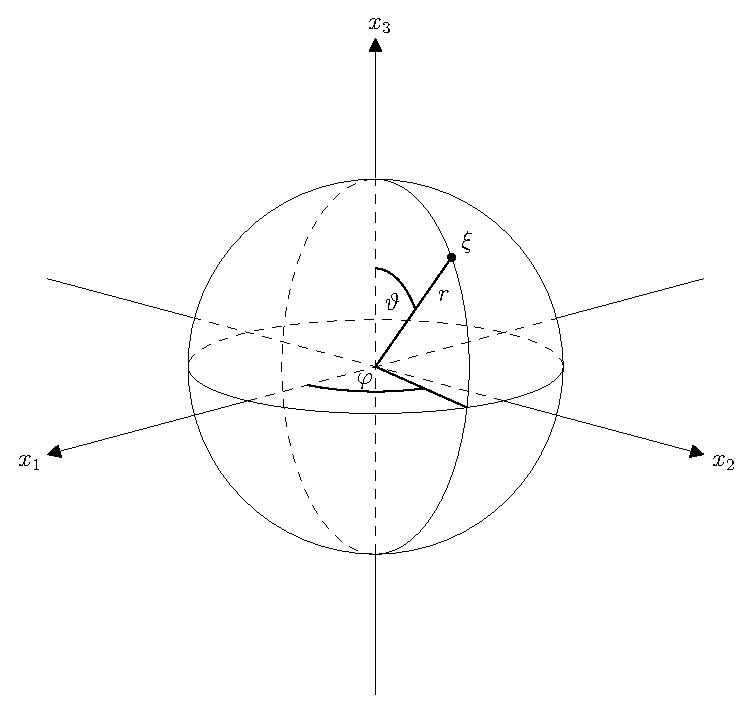
\includegraphics[height=12cm,width=12cm]{images/sphere}
  \caption{The spherical coordinate system in $\R^3$. Every point $\xi$ on a
  sphere with radius $r$ around the origin can be uniquely described by angles 
  $\vtheta$, $\vphi$ and the radius $r$. For $\vtheta = 0$ or
  $\vtheta = \pi$ the point $\xi$ coincides with the North or the South
  pole, respectively.}
  \label{sphere}
\end{figure}

\section{Legendre-type functions}
\label{Basics:LegendreTypeFunctions}
In this section we shortly define \emph{Legendre Polynomials}, \emph{associated Legendre functions} 
and \emph{associated Legendre polynomials} and collect some basic properties. These functions play 
a major role in Fourier analysis on the sphere and are key for the algorithms related to Fourier 
expansions developed in this text.

The Legendre polynomials $P_k : \interv{[}{-1}{1}{]} \rightarrow \R$, $k \in \N_{0}$ 
as classical orthogonal polynomials are given by their corresponding 
\emph{Rodrigues-formula}
\begin{equation}
  \nonumber
  \fun{P_k}{x} = \frac{1}{2^k k!} \frac{\dx^k}{\dx x^k} \paren{x^2-1}^k.
\end{equation}
The corresponding three-term recurrence relation is
\begin{equation}
  \nonumber
  \paren{k+1}\fun{P_{k+1}}{x} = \paren{2k+1}x\fun{P_{k}}{x} -
  k\fun{P_{k-1}}{x},\ k \in \N.
\end{equation}

Furthermore one defines the associated Legendre functions $P_k^n : \interv{[}{-1}{1}{]} \rightarrow \R$, 
$n \in \NZ$, $k=n,n+1,\ldots$ as 
\begin{equation}
  \nonumber
  \fun{P_k^n}{x} := \paren{\frac{\paren{k-n}!}{\paren{k+n}!}}^{1/2}
  \paren{1-x^2}^{n/2} \frac{\dx^n}{\dx x^n} \fun{P_k}{x}.
\end{equation}
For fixed $n$ the functions $\set{P_{k}^n}_{k=n,n+1,\ldots}$ form a complete set of orthogonal functions 
for $\Ln{2}{\interv{[}{-1}{1}{]}}$ with
$$ \frac{1}{2} \int_{-1}^{1} \fun{P_{k}^n}{x} \fun{P_{l}^n}{x} \dx x = \frac{1}{2k+1} \delta_{k,l}.$$
Furthermore, associated Legendre functions fulfill the recurrence relation
\begin{eqnarray*}
  & & \fun{P_{n-1}^n}{x} := 0,\qquad \fun{P_{n}^n}{x} = \frac{((2n)!)}{2^n n!}^{1/2} \paren{1-x^2}^{n/2},\\
  & & \fun{P_{k+1}^n}{x} = v_{k}^n x \fun{P_{k}^n}{x} + w_{k}^n \fun{P_{k-1}^n}{x} \quad (k = n,n+1,\ldots),
\end{eqnarray*}
where
$$ v_{k}^n := \frac{2k+1}{((k-n+1)(k+n+1))^{1/2}}\; ,\qquad w_{k}^n := - \frac{((k-n)(k+n))^{1/2}}{((k-n+1)(k+n+1))^{1/2}}\; .$$
A simple but at the same time very important idea is to define the associated Legendre functions also for 
$k < n$ by means of the three-term recurrence relation
$$ \fun{P_{k+1}^n}{x} = \paren{\alpha_{k}^n x \beta_{k}^n} \fun{P_{k}^n}{x} + \gamma_{k}^n \fun{P_{k-1}^n}{x} $$
with
\begin{eqnarray*}
  \alpha_{k}^n & := & \left\{
    \begin{array}{ll}
      (-1)^{k+1} & \text{for}\ k < n,\\
      v_{k}^n    & \text{otherwise},
    \end{array}\right.\\
  \beta_{k}^n & := & \left\{
    \begin{array}{lll}
      1 & \text{for}\ k < n,\\
      0 & \text{otherwise},
    \end{array}\right.\\
  \gamma_{k}^n & := & \left\{
    \begin{array}{lll}
      0       & \text{for}\ k \leq n,\\
      w_{k}^n & \text{otherwise.}
    \end{array}\right.\\
\end{eqnarray*}
For even $n$ one sets 
$$ \fun{P_{-1}^n}{x} := 0,\ \fun{P_{0}^n}{x} := \sqrt{\frac{(2n)!}{2^n n!}}$$
and for odd $n$
$$ \fun{P_{0}^n}{x} := \fun{P_{1}^n}{x} := \sqrt{\frac{(2n)!}{2^n n!}} \paren{1-x^2}^{1/2}$$
respectively. For $k >= n$ these functions coincide with the associated Legendre functions as defined above. 
As a matter of fact, $P_{k}^n$ is a polynomial of degree $k$ for even $n$ while $\paren{1-x^2}^{-1/2}P_{k}^n$
is a polynomial of degree $k-1$ for odd $n$.

Based on the recurrence coefficients from Equation \eqref{} and introducing a shift parameter $c \in \NZ$, one 
defines the associated Legendre polynomials $\fun{P_{k}^n}{\cdot,c}$ by
\begin{eqnarray*}
  & & \fun{P_{-1}^n}{x,c} := 0,\ \fun{P_{0}^n}{x,c} := 1,\\
  & & \fun{P_{k+1}^n}{x,c} = \paren{\alpha_{k+c}^n x + \beta_{k+c}^n} \fun{P_{k}^n}{x,c} + \gamma_{k+c}^n \fun{P_{k-1}^n}{x,c}
\end{eqnarray*}
By induction one verifies the relation between associated Legendre functions and polynomials in the following lemma.
\begin{lemma}
  Let the functions $P_{k}^n$ and $\fun{P_{k}^n}{\cdot,c}$ be given as in Equation \eqref{} and 
  Equation \eqref{} respectively. Then it holds
  $$ \fun{P_{c+k}^n}{x} = \fun{P_{k}^n}{x,c} \fun{P_{c}^n}{x} + \gamma_{c}^n \fun{P_{k-1}^n}{x,c+1} \fun{P_{c-1}^n}{x}. $$
\end{lemma}

\newpage

They can be characterized in ways similar
to those for Legendre polynomials, for instance by the
corresponding Rodrigues-formula or a differential equation. They
play an important role in the definition of spherical harmonics.
Note that for $k = 0$, the associated Legendre functions coincide with 
the Legendre polynomials.
Now let $k,m,n \in \N_0$, $k \le \min\encl{\{}{m,n}{\}}$. Then the associated
Legendre functions fulfill the orthogonality condition
\begin{equation}
\nonumber
  \int_{-1}^{1} \fun{P_{m}^{k}}{t} \fun{P_{n}^{k}}{t}\;dt =
  \frac{2}{2n+1}\delta_{m,n}.
\end{equation}



%Starting with the {\it{Legendre polynomials}}
% $$
% P_{k}(x):= \frac{1}{2^k k!} \frac{\dx^k}{\dx x^k} (x^2-1)^k\quad (x
% \in [-1,1]; k \in \N_{0})\; ,
% $$
% we define the {\it{associated Legendre functions}} $P_{k}^n \; (n \in
% \N_{0}; k = n,n+1, \ldots )$ as\\
% \begin{eqnarray}
% \label{assi}
% P_{k}^n(x):=\left(\frac{(k-n)!}{(k+n)!} \right)^{1/2} (1-x^2)^{n/2}
% \frac{\dx^n}{\dx x^n} P_{k}(x)\quad (x \in [-1,1])\; .
% \end{eqnarray}
% For any fixed $n \in \N_{0}$, the functions $P_{k}^n (k=n,n+1,
% \ldots )$ form a complete orthogonal system in $L^2[-1,1]$ with
% $$
% \frac{1}{2} \int\limits_{-1}^1 P_{k}^n (x) P_{l}^n (x) \dx x =
% \frac{1}{2k+1} \delta_{k,l}\quad (n \in \N_{0}; k,l=n,n+1, \ldots )\; .
% $$
% Moreover, the associated Legendre functions fulfill the three-term
% recurrence relation
% $$
% P_{n-1}^n (x):=0,\qquad P_{n}^n
%(x)= \frac{((2n)!)}{2^n n!}^{1/2} (1-x^2)^{n/2}\; ,
%$$
%\begin{equation}
%    P_{k+1}^n (x)=v_{k}^n x P_{k}^n (x) + w_{k}^n P_{k-1}^n
%    (x)\quad (k=n,n+1, \ldots )
%    \end{equation}
%    with
%    $$
%    v_{k}^n:= \frac{2k+1}{((k-n+1)(k+n+1))^{1/2}}\; ,\qquad
%    w_{k}^n:= - \frac{((k-n)(k+n))^{1/2}}{((k-n+1)(k+n+1))^{1/2}}\; .
%    $$
%    A simple but powerful idea in \cite{postta97} is to define the
%    functions $P_{k}^n$  also for $k < n$.
%    This was done as follows.
%    For even $n$ we start with $P_{-1}^n:=0$ and $P_{0}^n (x):=
%    \frac{\sqrt{(2n)!}}{2^n n!}$ and for odd $n$ let $P_{0}^n
%    (x):=P_{1}^n (x):= 
%    \frac{\sqrt{(2n)!}}{2^n n!} (1-x^2)^{1/2}$. We introduce the
%    functions $P_{k}^n$ by the three-term recurrence relation
%\begin{eqnarray}\label{drei}
%    P_{k+1}^n (x) := (\alpha_{k}^n x+ \beta_{k}^n) P_{k}^n (x) +
%    \gamma_{k}^n P_{k-1}^n (x)
%    \end{eqnarray}
%with
%    $$
%    \begin{array}{lllll}
%        \alpha_{k}^n := \left\{\begin{array}{lll}
%        (-1)^{k+1} &\ \mbox{for}\ k < n,\\
%        v_{k}^n &\ \mbox{otherwise},
%    \end{array}\right.\\[3ex]
%    \beta_{k}^n := \left\{\begin{array}{lll}
%        1 &\ \mbox{for}\ k < n,\\
%        0 &\ \mbox{otherwise},
%    \end{array}\right.\\[3ex]
%    \gamma_{k}^n := \left\{\begin{array}{lll}
%        0 &\ \mbox{for}\ k \leq n,\\
%        w_{k}^n &\ \mbox{otherwise.}
%    \end{array}\right.\\
%        \end{array}
%        $$
% It is a fact, that $P_{k}^n$ is a polynomial of degree $k$
% for even $n$ and that $(1-x^2)^{-1/2} P_{k}^n$ is a polynomial of degree
% $k-1$ for odd $n$. Furthermore, these functions coincide with
% (\ref{assi}) for $k\ge n$.
%The main reason for defining $P_k^n$ also for $k<n$ is that this
%modification allows a stable computation of the Legendre function transform.



\section{Spherical Harmonics}
\label{Basics:SphericalHarmonics}

For harmonic analysis in $\R^3$ the complex exponentials $e^{i \V{\omega}^{\transp} \cdot}$ 
($\V{\omega} \in \R^3$) provide the standard Fourier basis. With respect to the sphere one derives
from Laplace's equation restricted to the sphere solutions forming an orthonormal basis similar to
complex exponentials. We begin by noting some facts on 
orthogonal Legendre polynomials and the closely related associated
Legendre functions. Based on this
foundation, we describe the function space of spherical harmonics
and how it is related to spherical approximation.

Concerning the generating series of the Legendre polynomials
\begin{equation}
\label{LengendreFunctionsAndSphericalHarmonics.LegendrePolynomials.PowerSeries}
  \fun{\phi}{h} := \sum_{n = 0}^{\infty} \fun{P_n}{t} h^n,\ t \in
  \interv{[}{-1}{1}{]}
\end{equation}
which is absolutely and uniformly convergent for $h \in
\interv{(}{-1}{1}{)}$, it holds
\begin{equation}
  \label{LengendreFunctionsAndSphericalHarmonics.LegendrePolynomials.SeriesExpansion}
    \sum_{n = 0}^{\infty} \fun{P_n}{t} h^n = \frac{1}{\sqrt{1-2ht+h^2}}.
\end{equation}
This follows from the ordinary differential equation
\begin{equation}
\label{LengendreFunctionsAndSphericalHarmonics.LegendrePolynomials.SeriesExplicit}
  \paren{1+h^2-2ht}\fun{\phi'}{h} = \paren{t-h}\fun{\phi}{h}
\end{equation}
obtained by differentiation with respect to $h$ and comparing coefficients in line with Equation
\eqref{LengendreFunctionsAndSphericalHarmonics.LegendrePolynomials.PowerSeries}. Using the initial 
condition $\fun{\phi}{0}=1$ this yields the unique solution in Equation
\eqref{LengendreFunctionsAndSphericalHarmonics.LegendrePolynomials.SeriesExplicit}.
From this result, the following identity follows easily:
\begin{equation}
  \sum_{n=0}^{\infty} \paren{2n+1} \fun{P_n}{t} h^n =
  \frac{1-h^2}{\paren{1-2ht+h^2}^{3/2}}.
\end{equation}

When $h$ is restricted to $\interv{(}{0}{1}{)}$, the function
$G_h:\interv{[}{-1}{1}{]} \rightarrow \R$, with
\begin{equation}
\label{PoissonKernel}
  \fun{G_h}{t} := \frac{1-h^2}{\paren{1-2ht+h^2}^{3/2}},
\end{equation}
is called \emph{Poisson kernel}. We refer 
to Figure \ref{LengendreFunctionsAndSphericalHarmonics.LegendrePolynomials.Figure.PoissonKernel}
for a visual impression and take notice of the fact that the parameter $h$
allows for controlling the concentration of the function's energy around
$t = 1$.

\begin{figure}[htb]
  \centering
  \includegraphics[height=9cm,width=12cm]{images/poisson}
  \caption{The Poisson kernel for different values of $h$. The $x$-axis is scaled
  linearly
  with respect to $\vtheta$ while the argument for the function is $t=\cos\vtheta$. Since the cosine
  function is monotone in the interval $\interv{[}{0}{\pi}{]}$, this yields a bijective mapping to
  the interval $\interv{[}{-1}{1}{]}$, where $\vtheta = 0$ and $\vtheta = \pi$ correspond to
  $t=1$ and $t=-1$. This is the fashion, this function will be used in further
  investigations. It can be seen clearly that the energy more and more concentrates around
  $\vtheta = 0$ as $h$ gets closer to 1.}
  \label{LengendreFunctionsAndSphericalHarmonics.LegendrePolynomials.Figure.PoissonKernel}
\end{figure}


We now introduce the function space of spherical harmonics, a key to the treatment of spherical approximation problems.
From Laplace's differential equation $\Delta f = 0$ in $\R^3$, one obtains in spherical coordinates
\begin{equation}
  \label{SphericalHarmonics.LaplaceEquation.SphericalCoordinates}
  \Delta f = \frac{\partial^2 f}{\partial r^2} + \frac{2}{r}\frac{\partial f}{\partial
  r} + \frac{1}{r^2 \sin \vtheta}\frac{\partial}{\partial \vtheta}\paren{\sin \vtheta \cdot \frac{\partial f}{\partial
  \vtheta}} + \frac{1}{r^2 \sin \vtheta}\frac{\partial^2}{\partial \vphi^2} = 0.
\end{equation}
Using an ansatz based on separation of variables and taking into account that $r = 1$, one obtains the solutions
\begin{equation}
  \label{LegendreFunctionsAndSphericalHarmonics.SphericalHarmonics}
  \begin{split}
    Y_{n,k}: \interv{[}{0}{\pi}{]}\times\interv{[}{0}{2\pi}{)} \rightarrow
    \C,\\
    \fun{Y_{n,k}}{\vtheta,\vphi} := \sqrt{\frac{2n+1}{4\pi}} 
    \fun{P_{n}^{\abs{k}}}{\cos \vtheta} e^{ik\vphi},
  \end{split}
\end{equation}
where $n \in \N_{0},\ k = -n,-n+1,\dots,n$.
An important result states that the functions $Y_{n,k}$ are contained in $\fun{\text{Harm}_n}{\twosphere}$.
Due to the separability one proves easily
that they also fulfill the orthogonality condition with respect to the standard scalar product on $\twosphere$:
\begin{equation}
\label{LengendreFunctionsAndSphericalHarmonics.SphericalHarmonics.Orthogonality1}
\scalarproduct{Y_{n,j}}{Y_{m,k}}_{\twosphere} = \delta_{j,k} \delta_{n,m}\end{equation}
If we now define $\mathcal{H}_n$ to be
$\text{Harm}_n\paren{\twosphere}$, then
for every $n \in \N_0$, the set
\begin{equation}
  \nonumber
  \pset{Y_{n,k}}{|}{-n \le k \le n}
\end{equation}
forms an orthonormal basis of $\mathcal{H}_n$, since $\dim \mathcal{H}_n =
2n+1$. Moreover, the spaces $\mathcal{H}_n$ are orthogonal
to each other and the set 
$$\pset{Y_{n,k}}{|}{n = 0,1,\dots,N,\ k = -n,-n+1,\dots,n},\ N \in
\N_0$$ provides an orthonormal basis for the space
$\bigoplus_{n=0}^{N}\mathcal{H}_n$ called
the space of \emph{spherical harmonics} of degree $N$.

At first glance, the restriction to homogeneous and harmonic polynomials
might exclude various functions from being as well representable
as in $\fun{\Pi_n}{\twosphere}$. But as a matter of fact these
spaces are identical, i.e. 
\begin{equation}
  \nonumber
    \fun{\Pi_N}{\twosphere} = \bigoplus_{n=0}^{N}\mathcal{H}_n.
\end{equation}

We finally mention the well-known addition theorem of
spherical harmonics that relates basis functions of
$\mathcal{H}_n$ and Legendre-polynomials.
For every $\fun{L^2}{\twosphere}$ orthonormal basis
$\set{Y_{n,k}}_{k=-n}^{n}$ of $\mathcal{H}_n$, it holds
\begin{equation}
\label{AdditionTheorem}
  \sum_{k=-n}^{n} \fun{Y_{n,k}}{\V{\xi}}
  \overline{\fun{Y_{n,k}}{\V{\eta}}} =
  \frac{2n+1}{4\pi}\fun{P_n}{\scalarproduct{\V{\xi}}{\V{\eta}}_{\twosphere}}.
\end{equation}


\chapter{Nonuniform Discrete Spherical Fourier Transforms}
\label{DSFT}

In this chapter, we present algorithms for the computation of discrete
spherical Fourier transforms for arbitrary node distributions. 
Section \ref{NFSFT:dsfts} introduces the notation and naming conventions
of discrete Fourier transforms on the sphere $\twosphere$. We discuss
a simple \emph{direct algorithm} for evaluating a \emph{spherical Fourier sum}
at arbitrary nodes. The mapping of spherical Fourier coefficients to function 
values on the sphere can be represented in matrix-vector notation as the
multiplication of a complex vector $\V{a}$ containing the spherical Fourier 
coefficients with the complex \emph{spherical Fourier matrix} 
$\V{Y}$ yielding the complex vector $\V{f}$ of function values, i.e. 
$\V{f} = \V{Y} \: \V{a}$. 
Section \ref{NFSFT:iDSFT} concerns the inverse problem, i.e. how spherical Fourier
coefficients might be computed from a set function values. We give inversion
formulae in matrix-vector notation involving the adjoint of the 
\emph{spherical Fourier matrix} $\V{Y}^{\h}$. 
The corresponding \emph{adjoint direct algorithm} for the multiplication of
a complex vector $\V{\tilde{a}}$ with the matrix $\V{Y}^{\h}$ is 
obtained in Section \ref{NFSFT:Factorization} by a factorization of the 
matrix $\V{Y}$ according to the direct algorithm.

The following two sections are based on previous work from 
\cite{postta97} and \cite{kupo02}:
Discrete polynomial transforms allow for the conversion of
discrete spherical Fourier transform into ordinary two-dimensional
discrete Fourier transforms. Section \ref{DSFT:FLFT} introduces
the fast Legendre function transform (FLFT) which builds the core
for the fast discrete spherical Fourier transform algorithms later 
on. We discuss numerical problems and describe a stabilization 
procedure to circumvent them in Section \ref{NFSFT:Stabilization}.

As for the direct algorithm, we give a formulation in matrix-vector notation 
with a real matrix $\V{T}$ representing the FLFT algorithm.
We derive the factorization of the matrix $\V{T}$ following the description of
the algorithm in Section \ref{DSFT:LinearAlgebra}. We aim at 
obtaining the \emph{transposed FLFT algorithm} derived in Section
\ref{NFSFT:transposedFLFT} by transposing the matrix factorization.

In combination with the two-dimensional NFFT algorithm, we are able 
to construct a fast approximative algorithm for the evaluation
of a spherical Fourier sum at arbitrary nodes as in \cite{kupo02},
and moreover, in analogy to the direct algorithm, also the corresponding
fast adjoint algorithm in Section \ref{NFSFT:NFSFT}.
We close the chapter with an analysis of numerical stability and runtime 
performance compared to the direct algorithm.

\section{Discrete spherical Fourier transforms}
\label{NFSFT:dsfts}

Let in this chapter be $M \in \NZ$ fixed, $N := 2^t$ the 
next greater power of two with respect to $M$, i.e. $t := 
{\ceil{\log_2 M}}$, and $\mathcal{X} := 
\paren{\vtheta_d,\vphi_d}_{d=0}^{D-1}$ for $D \in \N$
a set of nodes on $\twosphere$ called the \emph{sampling set}. 
As a special case, a \emph{spherical grid} 
$\mathcal{X}$ is a Cartesian product 
\[
  \mathcal{X} = \pset{\vtheta_{l}}{|}{l=0,\ldots,L-1} \times \pset{\vphi_{j}}{|}{j=0,\ldots,J-1} \quad \paren{J,L \in \N}
\]
with \emph{colatitudes} $\vtheta_{l} \in \interv{[}{0}{\pi}{]}$ and \emph{longitudes} $\vphi_{j} \in \interv{[}{0}{2\pi}{)}$.
We denote by $\mathcal{I}^M$ the index set
\[
  \mathcal{I}^M := \pset{\paren{k,n}}{|}{k=0,\ldots,M;\ n=-k,\ldots,k}
\]
of \emph{admissible} indices $(k,n)$, and by $f$ a function $f: \twosphere \rightarrow \C$, $f \in \fun{\Pol_{M}}{\twosphere}$, hence a polynomial in $\R^3$ of degree at most $M$ restricted to the unit sphere $\twosphere$.

Referring to Section \ref{Basics:SphericalHarmonics}, the function $f$ can be developed into 
an orthogonal expansion in terms of the $\Ln{2}{\twosphere}$-orthogonal basis of
spherical surface functions $\set{Y_{k}^n}_{(k,n) \in \mathcal{I}^M}$, i.e.
\begin{equation}
  \label{NFSFT:FourierExpansion} 
  f = \sum_{\paren{k,n} \in\mathcal{I}^M} \fun{a_k^n}{f} Y_{k}^n = \sum_{k=0}^M \sum_{n=-k}^k \fun{a_k^n}{f} Y_{k}^n = \sum_{n=-M}^M \sum_{k=\abs{n}}^M \fun{a_k^n}{f} Y_{k}^n.
\end{equation}  
Equation \eqref{NFSFT:FourierExpansion} is the \emph{spherical Fourier sum} or 
\emph{spherical Fourier expansion} of the function $f$ and $M$ is called the 
\emph{bandwidth}. Likewise, $f$ is said to be a \emph{bandlimited} function 
on $\twosphere$ with bandwidth $M$. So far, the nomenclature alludes to the 
usual conception of 'classical' Fourier analysis and signal theory on the 
unit circle $\mathbb{S}^1$. This chapter will deal with algorithms related 
to \eqref{NFSFT:FourierExpansion} subsumed under the topic \emph{discrete 
spherical Fourier transform (DSFT)} which can be regarded as the spherical 
analog of the \emph{discrete Fourier transform (DFT)} for the unit circle 
$\mathbb{S}^1$. Furthermore, the generalizing idea of \emph{irregular sampling}, 
referring to arbitrary sampling sets $\V{\mathcal{X}}$, is incorporated into 
the algorithms. In order to form a concise notion, one needs on the one hand 
to keep the widespread and accepted vocabulary from 'classical' Fourier 
analysis, but on the other hand, to introduce modified denotations in order 
to reflect the generalized conception. Speaking of the DFT for the unit 
circle $\mathbb{S}^1$, one refers to the transformation of a sequence of $K \in \N$ 
complex numbers $\paren{g_{k}}_{k=0}^{K-1}$ into the sequence of $K$ 
complex numbers $\paren{\hat{g}_{k}}_{k=0}^{K-1}$ according to the formula
\[
  \hat{g}_{k} := \sum_{j=0}^{K-1} g_{j} \e^{-2\pi\im \frac{jk}{K}} \quad \paren{k=0,\ldots,K-1}.
\]
The numbers $g_{j}$ can be regarded as samples of a bandlimited 
signal $g: \mathbb{S}^1 \rightarrow \C$ at uniformly distributed nodes 
$\vphi_{k} := \frac{2\pi k}{K}$ whereas the numbers $\hat{g}_{k}$
can be interpreted as the \emph{frequencies} contained in the signal $g$.
A translation of this concept to the sphere $\twosphere$ and the incorporation 
of irregular sampling imposes a deviation from the standard notation. 

We refer to the 
\emph{nonuniform discrete spherical Fourier transform (NDSFT)} as the 
transformation of spherical Fourier coefficients 
$\paren{\fun{a_{k}^n}{f}}_{(k,n) \in \mathcal{I}^M}$ 
of a bandlimited function $f$ into function samples 
$\paren{\fun{f}{\vtheta_{d},\vphi_{d}}}_{d=0}^{D-1}$ on an arbitrary sampling 
set $\mathcal{X}$. The fast related algorithm presented in this chapter is 
named \emph{nonuniform fast spherical 
Fourier transform (NFSFT)}. Owing to the generalization for arbitrary 
sampling sets, the inverse transformation, hence
the recovery of the spherical Fourier coefficients 
$\paren{\fun{a_{k}^n}{f}}_{(k,n) \in \mathcal{I}^M}$ from the function samples
$\paren{\fun{f}{\vtheta_{d},\vphi_{d}}}_{d=0}^{D-1}$ is an ill-posed problem, 
since it might be neither properly nor uniquely defined.
We therefore preserve the term DSFT for the case when 
spherical sampling grids $\mathcal{X}$ are used which allow for the 
reconstruction of the spherical Fourier coefficients from the corresponding 
function samples.

The index $k$ will always denote the degree and $n$ always the order with respect to the functions $Y_{k}^n$. The spherical Fourier coeffcients $a_{k}^n$ may be ordered 
in different ways. We use
\begin{equation}
  \label{Basics:Ordering}
  a_{M}^{-M},\: a_{M-1}^{-(M-1)},\: a_{M}^{-(M-1)},\: a_{M-2}^{-(M-2)},
  \: \ldots,\: a_{M-1}^{M-1},\: a_{M}^{M-1},\: a_{M}^{M}
\end{equation}
as the standard ordering, i.e. first by order $n$ then by degree $k$.
From a linear algebra point of view, evaluating the function $f$ on the 
sampling set $\mathcal{X}$ corresponds to a matrix-vector product
\[ 
  \V{f}_{\mathcal{X}} = \V{Y}_{\mathcal{X}} \; \V{a}
\]
with
\begin{equation}
  \nonumber
  \begin{split}
    \V{f}_{\mathcal{X}} & := \paren{f_d}_{d=0}^{D-1} \in \C^{D},\ f_{d} := \fun{f}{\vtheta_{d},\vphi_{d}},\\
    \V{Y}_{\mathcal{X}} & := \paren{\fun{Y_k^n}{\vtheta_d,\vphi_d}}_{d=0,\ldots,D-1; 
      \paren{k,n} \in \mathcal{I}^M} \in \C^{D \times \paren{M+1}^2},\\
    \V{a} & := \paren{a_k^n}_{\paren{k,n} \in \mathcal{I}^M} \in \C^{\paren{M+1}^2}.
  \end{split}
\end{equation}
If not specified otherwise, the vector $\V{a}$ contains the Fourier 
coeffcients $\paren{a_{k}^n}_{(k,n) \in \mathcal{I}^M}$ in the 
standard ordering \eqref{Basics:Ordering}, and the columns of 
$\V{Y}_{\mathcal{X}}$ are ordered accordingly. We drop the 
index $\mathcal{X}$ for $\V{f}_{\mathcal{X}}$ and 
$\V{Y}_{\mathcal{X}}$ where appropriate.
%We drop the indices $\mathcal{X}$ and $M$ where appropriate, i.e. where they could be chosen arbitrarily or are obvious from the 
%context and write $\V{f} = \V{Y} \; \V{a}$ instead. 
Furthermore, we introduce the notation
\begin{equation}
  \nonumber
  \V{a}^{n} := \paren{a_{k}^{n}}_{k=|n|}^{M} \in \C^{M-|n|+1} \quad \paren{n=-M,\ldots,M},
\end{equation} 
for subvectors of $\V{a}$. If $\mathcal{X}$ is a spherical grid, the standard ordering of the nodes is first by longitude $\vphi_{j}$ and then by 
colatitude $\vtheta_{l}$. 
Furthermore, we use double subscripts $l,j$ to denote $\V{f}_{l,j} := \fun{f}{\vtheta_{l},\vphi_{j}}$.

A first 'naive' approach to evaluating $f$ on the sampling set $\mathcal{X}$ according to \eqref{NFSFT:FourierExpansion} would be to compute first all $(M+1)^2D$
entries of the matrix $\V{Y}_{\mathcal{X}}$ and then perform the matrix-vector multiplication $\V{Y} \: \V{a}$ the standard way. This would lead to an $\bigo{M^3D}$ algorithm, since the evaluation of a single function 
$Y_{k}^n$ at a single node already requires $\bigo{M}$ flops.
But one can do better: Algorithm \ref{NFSFT:directDSFT}, referred 
to as \emph{direct nonuniform discrete spherical Fourier transform (NDSFT)}, computes 
for every $\paren{\vtheta_{d},\vphi_{d}} \in \mathcal{X}$ first the sums 
\begin{equation}
  \label{NFSFT:directDSFT:firstSum}
  b^{n}_{d} := \sum_{k=\abs{n}}^M a_{k}^n \fun{P_{k}^{\abs{n}}}{\cos\vtheta_{d}} \quad \paren{n=-M,\ldots,M}. 
\end{equation}
Here, we can employ the \emph{Clenshaw algorithm} (see Algorithm \ref{NFSFT:Algorithm:Clenshaw} and \cite{prtevefl}) 
by using the three-term recurrence \eqref{Basics:AssociatedLegendreDefinition}
for associated Legendre functions. We finally compute
\begin{equation}
  \label{NFSFT:directNDSFT:secondSum}
  \fun{f}{\vtheta_{d},\vphi_{d}} = \sum_{n=-M}^M b^{n}_d \e^{\im n \vphi_{d}}
\end{equation}
directly. Each application of the Clenshaw algorithm for fixed $n$ to evaluate \eqref{NFSFT:directDSFT:firstSum} needs $\bigo{M}$ 
flops, summing up to $\bigo{M^2}$ flops for $n = -M,\ldots,M$. In 
total, we have an $\bigo{M^2 D}$ algorithm for the evaluation of $f$ on the sampling set $\mathcal{X}$ and gained an order of complexity with respect to $M$. 
\begin{algorithm}[tb]
  \caption{Clenshaw Algorithm for \eqref{NFSFT:directDSFT:firstSum}}
  \label{NFSFT:Algorithm:Clenshaw}    
  \begin{algorithmic}
    \STATE  Input: $M \in \NZ$, $n \in \Z$ with $\abs{n} \le M$, $\V{a}^n$, $x := \cos\vtheta_{d} \in \interv{[}{-1}{1}{]}$
    \STATE
    \FOR {$k=M,\ldots,\abs{n}+2$} 
      \STATE $a_{k-1}^n := a_{k-1}^n + \paren{\alpha_{k}^{|n|} x + \beta_{k}^{|n|}} a_{k}^n$
      \STATE $a_{k-2}^n := a_{k-2}^n + \gamma_{k}^{|n|} a_{k}^n$
    \ENDFOR
    \STATE $a_{\abs{n}}^n := a_{\abs{n}}^n + \paren{\alpha_{\abs{n}+1}^{|n|} x + \beta_{\abs{n}+1}^{|n|}} a_{\abs{n}+1}^n$\\[0.5ex]
    \STATE $b_{d}^n := \frac{\sqrt{(2|n|)!}}{2^{|n|} |n|!} \paren{1-x^2}^{|n|/2} a_{\abs{n}}^n$
    \STATE
    \STATE Output: $b_{d}^n$
    \STATE Complexity: $\bigo{M}$ flops
\end{algorithmic}
\end{algorithm}
\begin{algorithm}[tb]
  \caption{Direct DSFT}
  \label{NFSFT:directDSFT}    
  \begin{algorithmic}
    \STATE  Input: $M \in \NZ$, $D \in \N$, $\V{a}$, $\mathcal{X}$
    \STATE
    \FOR {$d=0,\ldots,D-1$} 
      \STATE $f_{d} := 0$
      \FOR {$n=-M,\ldots,M$} 
        \STATE Compute $b^{n}_d$ by Algorithm \ref{NFSFT:Algorithm:Clenshaw},
        \STATE $f_{d} := f_{d} + b^n_d \e^{\im n \vphi_{d}}$
      \ENDFOR
    \ENDFOR
    \STATE
    \STATE Output: $\V{f}_{\mathcal{X}}$
    \STATE Complexity: $\bigo{M^2 D}$ flops
\end{algorithmic}
\end{algorithm}

For special sampling sets one can exploit the grid 
structure and employ FFT techniques for the sums \eqref{NFSFT:directNDSFT:secondSum} if the nodes $\varphi_{d}$ are distributed uniformely 
(see \cite{drhe}, \cite{postta97} and \cite{kupo02}). 

%\citelist{\cite{Mo99} \cite{postta97} \cite{roty} \cite{suta}}

\section{Computing Fourier Coeffcients from Function Samples}
\label{NFSFT:iDSFT}
A \emph{discrete Fourier transform (DFT)} on the unit circle $\mathbb{S}^1$, identified with the interval $[0,2\pi)$, 
of length $K \in \NZ$ can be represented as a maxtrix-vector product
$\V{g} = \V{F} \: \V{\hat{g}}$ with
\[
 \V{F} := \paren{\e^{2 \pi i \frac{kj}{K}}}_{k,j = 0}^{K-1} \in 
 \C^{K \times K},\ \V{\hat{g}},\:\V{g} \in \C^{K},
\]
The unitary Fourier matrix $\V{F}$ yields the inversion formula
\begin{equation}
  \label{NFSFT:DFTInversion}
  \V{\hat{g}} = \V{F}^{\h} \: \V{g}
\end{equation}
immediately. The DFT is a linear mapping that evaluates a 
trigonometric polynomial of degree $K$
\[
  g := \sum_{k=0}^{K-1} \fun{\hat{g}}{k} \e^{2 \pi \im k \vphi}
\]
at uniformely distributed nodes $\paren{\vphi_{d}}_{d=0}^{K-1}$ with $\vphi_{d} := \frac{d}{K} \in \mathbb{S}^1$. 
For an arbitrary sampling set $\mathcal{Y}$, the associated Fourier matrix 
$\V{F}_{\mathcal{Y}}$ is in general no longer unitary. 
Depending on the number of Fourier coefficients and the number of nodes,
$\V{F}_{\mathcal{Y}}$ is moreover no longer square.

Having defined the NDSFT as the evaluation of a bandlimited function $f \in 
\fun{\Pi_{M}}{\twosphere}$ on an \emph{arbitrary} 
sampling set $\mathcal{X}$ on $\twosphere$, arises immediately the question 
whether in the spherical case, there exist sampling sets $\mathcal{X}$ allowing for an inversion formula similar to \eqref{NFSFT:DFTInversion}.
The answer is affirmative, but in general, the number of nodes needed exceeds the number of Fourier coefficients to be computed, 
i.e. $\V{Y}_{\mathcal{X}}$ is not square.

We want to recover the spherical Fourier coefficients $\paren{a_{k}^n}_{(k,n) \in \mathcal{I}^M}$ of a bandlimited function $f \in \fun{\Pi_{M}}{\twosphere}$
from samples $\V{f}_{\mathcal{X}}$ on a sampling set $\mathcal{X} \subset \twosphere$. 
They spherical Fourier coefficients $a_{k}^n$ are given by the inner products
\[
  a_{k}^n = \scalarproduct{f}{Y_{k}^n}_{\Ln{2}{\twosphere}} = \int_{0}^{2\pi} \int_{0}^{\pi} 
  \fun{f}{\vtheta,\vphi} \overline{\fun{Y_{k}^n}{\vtheta,\vphi}} \sin \vtheta 
  \; \dx \vtheta \; \dx \vphi.
\]
By separating the integrand with respect to the integration variables $\vtheta$ and $\vphi$, we obtain
\begin{align*}
  a_{k}^n & = \int_{0}^{2\pi} \int_{0}^{\pi} \fun{f}{\vtheta,\vphi} \fun{P_{k}^{\abs{n}}}{\cos \vtheta} \e^{-\im n \vphi} \sin \vtheta \; \dx \vtheta \; \dx \vphi\\
          & = \int_{0}^{\pi} \fun{P_{k}^{\abs{n}}}{\cos \vtheta} \sin \vtheta \; \int_{0}^{2\pi} \fun{f}{\vtheta,\vphi} \e^{-\im n \vphi} \; \dx \vphi \; \dx \vtheta.
\end{align*}
For the integrals
\[
  \fun{f_{n}}{\vtheta} := \int_{0}^{2\pi} \fun{f}{\vtheta,\vphi} \e^{-\im n \vphi} \; \dx \vphi
\]
we have the quadrature rule
\[ 
  \fun{f_{n}}{\vtheta} = \frac{1}{2(M+1)} \sum_{j=0}^{2M+1} \fun{f}{\vtheta,\vphi_{j}} \e^{-\im n \vphi_{j}}
\]
with the nodes
\[ 
  \vphi_{j} := \frac{j\pi}{M+1} \quad \paren{j=0,\ldots,2M+1}. 
\]
This holds (cf. \cite[Chapter X]{Zy}) by taking into account that for fixed $\vtheta$, the function
\[
  \fun{f}{\vtheta,\cdot} = \sum_{(k,n) \in \mathcal{I}^M} a_{k}^n
  \fun{Y_{k}^n}{\vtheta,\cdot} = \sum_{n=-M}^{M} 
  \left(\sum_{k=\abs{n}}^M a_{k}^n 
  \fun{P_{k}^{\abs{n}}}{\cos \vtheta}\right) \e^{-\im n \: \cdot}
\]
is a trigonometric polynomial of degree $M$ with Fourier coefficients
\[
  \fun{\paren{\fun{f}{\vtheta,\cdot}}^{\wedge}}{n} := \sum_{k=\abs{n}}^M a_{k}^n \fun{P_{k}^{\abs{n}}}{\cos \vtheta}.
\]
It remains to compute
\[
  a_{k}^n = \int_{0}^{\pi} \fun{P_{k}^{\abs{n}}}{\cos \vtheta} \fun{f_{n}}{\vtheta} \sin \vtheta \; \dx \vtheta = 
  \int_{-1}^1 \fun{P_{k}^{\abs{n}}}{x} \fun{f_{n}}{\arccos x} \; \dx x.
\]
By verifying that $\fun{P_{k}^{\abs{n}}}{x} \fun{f_{n}}{\arccos x}$ is an algebraic polynomial of degree at most $2M+1$, 
we are free to use different quadrature rules for the remaining integrals. We 
first mention the \emph{Gauss-Legendre} quadrature rule
\[
  \int_{0}^{\pi} \fun{P_{k}^{\abs{n}}}{\cos \vtheta} \fun{f_{n}}{\vtheta} \sin \vtheta \; \dx \vtheta = \sum_{l=0}^{M} w_{l}^{\gl} \fun{P_{k}^{\abs{n}}}{\cos \vtheta_{l}^{\gl}} \fun{f_{n}}{\vtheta_{l}^{\gl}} 
\]
with nodes $\paren{\vtheta_{l}^{\gl}}_{l=0}^M$ and weights $\paren{w_{l}^{\gl}}_{l=0}^M$ as described, for example in \cite{boehme02}. 
We note that the $M+1$ nodes $\paren{\vtheta_{l}^{\gl}}_{l=0}^{M}$ can be computed as the eigenvalues of the \emph{Jacobi matrix} for the orthogonal 
Legendre polynomials $P_{k}$. The weights $\paren{w_{l}^{\gl}}_{l=0}^{M}$ are obtained from the corresponding eigenvectors.

A second idea is to employ a \emph{Clenshaw-Curtis} quadrature rule (see \cite{dara}, pp. 86)
\[
  \int_{0}^{\pi} \fun{P_{k}^{\abs{n}}}{\cos \vtheta} \fun{f_{n}}{\vtheta} \sin \vtheta \; \dx \vtheta = \sum_{l=0}^{2M} w_{l}^{\cc} \fun{P_{k}^{\abs{n}}}{\cos \vtheta_{l}^{\cc}} \fun{f_{n}}{\vtheta_{l}^{\cc}}
\]
where $\vtheta_{l}^{\cc} = \frac{l\pi}{2M}$ are the \emph{Chebyshev nodes}.
This quadrature rule uses almost twice as many points as the Gauss-Legendre quadrature rule but allows for an easy and fast online computation of the nodes $\vtheta_{l}^{\cc}$ and weights $w_{l}^{\cc}$. The weights $ w_{l}^{\cc}$ 
are given by
\[ 
  w_{l}^{\cc} := \frac{\varepsilon_{l}^{2M}}{M} \sum_{j=0}^{M}
  \varepsilon_{j}^{M} \frac{-2}{4j^2-1} \cos\frac{lj\pi}{M} 
  \quad \paren{l=0,\ldots,2M},
\]
with $\varepsilon_{0}^{M} := \varepsilon_{M}^{M} := \frac{1}{2}$, 
$\varepsilon_{l}^{M} := 1$, $l = 1,\ldots,M-1$.
Finally, the identities 
\begin{equation}
  \label{NFSFT:iDSFT}
  \begin{split}
    a_{k}^n & = \frac{1}{2(M+1)} \sum_{j=0}^{2M+1} \sum_{l=0}^{M} w_{l}^{\gl} \fun{f}{\vtheta_{l}^{\gl},\vphi_{j}} \overline{\fun{Y_{k}^n}{\vtheta_{l}^{\gl},\vphi_{j}}},\\
    a_{k}^n & = \frac{1}{2(M+1)} \sum_{j=0}^{2M+1} \sum_{l=0}^{2M} w_{l}^{\cc} \fun{f}{\vtheta_{l}^{\cc},\vphi_{j}} 
  \overline{\fun{Y_{k}^n}{\vtheta_{l}^{\cc},\vphi_{j}}}
  \end{split}
\end{equation}
follow. Associated with these quadrature formulae, we define the spherical grids
\begin{eqnarray*}
  \mathcal{X}^{\gl} & := & \paren{\vtheta_{l}^{\gl},\vphi_{j}}_{j=0,\dots,2(M+1)-1;l=0,\dots,M},\\
  \mathcal{X}^{\cc} & := & \paren{\vtheta_{l}^{\cc},\vphi_{j}}_{j=0,\dots,2(M+1)-1;l=0,\dots,2M},
\end{eqnarray*}
and refer to $\mathcal{X}^{\gl}$ as the \emph{Gauss-Legendre sampling grid of degree M} and to $\mathcal{X}^{\cc}$ as the 
\emph{Clenshaw-Curtis sampling grid of degree M}. They are illustrated in Figure \ref{quadrature}.
\begin{figure}[tb]
  \centering
  \includegraphics[width=0.6\textwidth]{images/quadrature}
  \caption{The sampling grids $\mathcal{X}^{\gl}$ (black dots) and $\mathcal{X}^{\cc}$ (gray dots) for $M=7$.}
  \label{quadrature}
\end{figure}
Note that in contrast to the Gauss-Legendre sampling set $\mathcal{X}^{\gl}$,
the Clenshaw-Curtis sampling set $\mathcal{X}^{\cc}$ always contains the poles.
We now immediately obtain the corresponding inversion formulae in matrix-vector notation
\begin{equation}
  \label{NFSFT:InversionFormula}
  \begin{split}
    \V{a} & = \V{Y}_{\mathcal{X}^{\gl}}^{\h} \: \V{W}^{\gl} \:
    \V{f}_{\mathcal{X}^{\gl}},\quad \V{W}^{\gl} := \V{I}_{2M+2} 
    \otimes \diag\paren{\paren{w_{l}^{\gl}}_{l=0}^M},\\
    %\label{NFSFT:InversionFormulaCC}
    \V{a} & = \V{Y}_{\mathcal{X}^{\cc}}^{\h} \: \V{W}^{\cc} \:
    \V{f}_{\mathcal{X}^{\cc}},\quad \V{W}^{\cc} := \V{I}_{2M+2} 
    \otimes \diag\paren{\paren{w_{l}^{\cc}}_{l=0}^{2M}}.
  \end{split}  
\end{equation}  
An algorithm for the multiplication with the adjoint spherical Fourier matrix $\V{Y}^{\h}$ is 
the key for the implementation of a reconstruction algorithm according to 
\eqref{NFSFT:InversionFormula}. Evaluating the
matrix-vector product the standard way, i.e. row-wise with respect to the matrix $\V{Y}^{\h}$, 
a first approach 
would be to successively compute the Fourier coefficients $a_{k}^n$ by the quadrature formulae 
\eqref{NFSFT:iDSFT} for all $\paren{k,n} \in \mathcal{I}^M$ employing the Clenshaw 
algorithm for the evaluation of the spherical surface functions $Y_{k}^n$. But we would only have an 
$\bigo{M^3 D}$ algorithm due to the fact that the Clenshaw algorithm would now be 
applied to each function $Y_{k}^n$ seperately instead of evaluating a whole linear 
combination as in Algorithm \ref{NFSFT:directDSFT}. 
We would end up with an $\bigo{M^3 D}$ algorithm for the NDSFT, too, if we 
evaluated the matrix $\V{Y}$ componentwise and then performed the matrix-vector multiplication 
as usual. But Algorithm \ref{NFSFT:directDSFT} for the direct NDSFT implies a factorization of 
the matrix $\V{Y}$ into a product of matrices, representing the distinct steps therein.
By taking the adjoint factorization, we obtain a factorization of $\V{Y}^{\h}$ immediately, and 
thus are able to construct an algorithm with the same arithmetic complexity $\bigo{M^2 D}$.

\section{A Factorization of the Spherical Fourier Matrix}
\label{NFSFT:Factorization}

Since the adjoint matrix $\V{Y}^{\h}$ is not generally the inverse of $\V{Y}$, i.e. $\V{Y}^{\h} 
\neq \V{Y}^{-1}$, we use $\V{\tilde{a}}$ and $\V{\tilde{f}}$ instead of $\V{a}$ and $\V{f}$ 
in the matrix-vector notation to make clear 
that we do not mean the inverse transform here. The product
\[
  \V{\tilde{a}} = \V{Y}^{\h} \: \V{\tilde{f}}
\]
yields coefficients $\V{\tilde{a}} = \paren{\tilde{a}_{k}^n}$ that 
we refer to as \emph{pseudo-Fourier coefficients}. Similarly, we speak of
\emph{pseudo-function samples} $\V{\tilde{f}} = (\tilde{f}_{d})_{d=0}^{D-1}$ as input values,
instead.
In order to abtain the $\bigo{M^2D}$ algorithm for the adjoint matrix-vector product, 
we first derive the factorization of the matrix $\V{Y}$ according to Algorithm 
\ref{NFSFT:directDSFT}. The matrix $\V{Y}$ can be written as
\[
  \V{Y} = 
    \left[\begin{array}{c}
      \V{E}_{0}\\
      \V{E}_{1}\\
      \vdots\\
      \V{E}_{D-1}
    \end{array}\right], \quad \V{E}_{d} \in \C^{1 \times (M+1)^2} \quad \paren{d=0,\ldots,D-1}.
\]
Each matrix $\V{E}_{d}$ evaluates the function $f$ at a node $\paren{\vtheta_{d},\vphi_{d}}$ according to 
\[
  \fun{f}{\vtheta_{d},\vphi_{d}} = \sum_{n=-M}^M \sum_{k=\abs{n}}^M a_k^n \fun{Y_{k}^n}{\vtheta_{d},\vphi_{d}}.
\]
Let now $d$ be fixed. The direct NDSFT algorithm begins by evaluating the sums
\[
  b^{n}_{d} = \sum_{k=\abs{n}}^M a_{k}^n \fun{P_{k}^{\abs{n}}}{\cos\vtheta_{d}} \quad \paren{n=-M,\ldots,M}, 
\]
which corresponds to computing
\[
  \left(\begin{array}{c}
    b^{-M}_{d}\\[1ex]
    b^{-(M-1)}_{d}\\[-1ex]
    \vdots\\[1ex]
    b^{M}_{d}
  \end{array}\right)
  =
  \left[\begin{array}{cccc}
    \V{C}^{-M}_{d} &                    &        &               \\
                   & \V{C}^{-(M-1)}_{d} &        &               \\
                   &                    & \ddots &               \\
                   &                    &        & \V{C}^{M}_{d} 
  \end{array}\right]
  \:
  \left[\begin{array}{c}
    \V{a}^{-M}\\
    \V{a}^{-(M-1)}\\[-1ex]
    \vdots\\[1ex]
    \V{a}^{M}
  \end{array}\right],
\]
where each matrix $\V{C}^{n}_{d} \in \R^{1 \times (M-n+1)}$ for $n = -M,\ldots,M$ realizes the Clenshaw algorithm 
(see Algorithm \ref{NFSFT:Algorithm:Clenshaw}) for \eqref{NFSFT:directDSFT:firstSum} acting on the subvector $\V{a}^n$ of $\V{a}$.
The matrices $\V{C}_{d}^n$ can be further decomposed according to the number of steps in the Clenshaw algorithm by
\begin{align*}
  \V{C}^{n}_{d}       
  & := \frac{\sqrt{(2|n|)!}}{2^{|n|} |n|!} 
       \paren{1-\cos^2\vtheta_{d}}^{|n|/2}
       \prod_{l=1}^{M-|n|} \V{C}_{d,l}^{n},\\
  \V{C}_{d,l}^{n}     
  & := \encl{[}{\V{I}_{l}, \V{\tilde{e}}_{d,l}}{]} \in \R^{l \times (l+1)} 
  & \quad \paren{l=1,\ldots,M-|n|},\\
  \V{\tilde{e}}_{d,1} 
  & := \paren{\alpha_{|n|}^n \vtheta_{d} + \beta_{|n|}^n}^{\transp} 
       \in \R^{1},\\
  \V{\tilde{e}}_{d,l} 
  & := \paren{0,0,\ldots,\gamma_{l+|n|-1}^n,\alpha_{l+|n|-1}^n 
       \vtheta_{d} + \beta_{l+|n|-1}^n}^{\transp} \in \R^{l} 
  & \quad \paren{l=2,\ldots,M-\abs{n}}.
\end{align*}
Finally, we compute the sum
$%\[
  f_{d} = \sum_{n=-M}^M b^{n}_{d} \e^{\im n \vphi_{d}}
$ %\]
by forming the inner product
\[
  f_{d} 
  = 
%  \V{E}_{d}
%  \:
%  \V{a}
%  =
  \paren{\e^{\im (-M) \vphi_{d}},\e^{\im (-(M-1)) \vphi_{d}},\ldots,\e^{\im M \vphi_{d}}}
  \:   
  \left(\begin{array}{c}
    b^{-M}_{d}\\
    b^{-(M-1)}_{d}\\
    \vdots\\
    b^{M}_{d}
  \end{array}\right).
\]
This gives the representation
\[
  \V{E}_{d} = \paren{\e^{\im (-M) \vphi_{d}},\e^{\im (-(M-1)) \vphi_{d}},\ldots,\e^{\im M \vphi_{d}}} \:  
  \left[\begin{array}{cccc}
    \V{C}^{-M}_{d} &                    &        &               \\
                   & \V{C}^{-(M-1)}_{d} &        &               \\
                   &                    & \ddots &               \\
                   &                    &        & \V{C}^{M}_{d} 
  \end{array}\right].
\]

\section{Adjoint and Inverse DSFT}

We obtain the sought algorithm for the adjoint transform directly from the factorization 
given in the last section. We have to evaluate $\V{\tilde{a}} = \V{Y}^{\h} \: \V{\tilde{f}}$, i.e.
\begin{equation}
  \label{NFSFT:adjointNDSFTFactorization2}
  \V{\tilde{a}}
  =
  \encl{[}{
    \V{E}_{0}^{\h},
    \V{E}_{1}^{\h},
    \ldots,
    \V{E}_{D-1}^{\h}
  }{]}
  \:
  \left(\begin{array}{c}
    \tilde{f}_{0}\\
    \tilde{f}_{1}\\
    \vdots\\
    \tilde{f}_{D-1}
  \end{array}\right). 
\end{equation}
This decomposition corresponds to the evaluation of the matrix-vector product in a, say, nonstandard 
way, by traversing the 
matrix column-wise instead of row-wise. After each column $\V{E}_{d}^{\h}$, the result vector is updated with the portion due 
to the matrix-vector product $\V{\tilde{a}}_{d} := \V{E}^{\h}_{d} \: \tilde{f}_{d}$. We obtain the vector $\V{\tilde{a}}$ as
\begin{equation}
  \label{}
  \V{\tilde{a}} = \V{\tilde{a}}_{0} + \V{\tilde{a}}_{1} + \ldots + \V{\tilde{a}}_{D-1}.
\end{equation}
For a particular vector $\V{\tilde{a}}_{d}$, we have
\begin{equation}
  \label{NFSFT:adjointNDSFTFactorization}
  \V{\tilde{a}}_{d}
  =
  \left[\begin{array}{cccc}
    {\V{C}^{-M}_{d}}^{\transp} &                               &        &                           \\
                              & {\V{C}^{-(M-1)}_{d}}^{\transp} &        &                           \\
                              &                                & \ddots &                           \\
                              &                                &        & {\V{C}^{M}_{d}}^{\transp} 
  \end{array}\right]
  \:
  \left(\begin{array}{c}
    \e^{\im M \vphi_{d}}\\
    \e^{\im (M-1) \vphi_{d}}\\[-1ex]
    \vdots\\[1ex]
    \e^{\im (-M) \vphi_{d}}
  \end{array}\right)
  \:
  f_{d}.
\end{equation}
A multiplication with a transposed matrix ${\V{C}^{n}_{d}}^{\transp}$ realizes a 
\emph{transposed Clenshaw algorithm} summarized in Algorithm \ref{NFSFT:transposedClenshaw}. 
The complete algorithm can be constructed directly from \eqref{NFSFT:adjointNDSFTFactorization2} and 
\eqref{NFSFT:adjointNDSFTFactorization} and is given in Algorithm \ref{NFSFT:adjointDSFT}.
\begin{algorithm}[tb]
  \caption{Transposed Clenshaw Algorithm}
  \label{NFSFT:transposedClenshaw}    
  \begin{algorithmic}
    \STATE  Input: $M \in \NZ$, $n \in \NZ$ with $\abs{n} \le M$, $\tilde{b}^n_{d}$, $x := \cos\vtheta_{d} \in \interv{[}{-1}{1}{]}$
    \STATE
    \STATE $\tilde{a}_{d,\abs{n}-1}^n := 0$
    \STATE $\tilde{a}_{d,\abs{n}}^n := \frac{\sqrt{(2|n|)!}}{2^{|n|} |n|!}^{1/2} \paren{1-x^2}^{|n|/2} \tilde{b}^n_{d}$
    \FOR {$k=\abs{n}+1,\ldots,M$} 
      \STATE $\tilde{a}_{d,k}^n := \paren{\alpha_{k}^n\vtheta_{d} + \beta_{k}^n}\tilde{a}_{d,k-1}^n + \gamma_{k}^n \tilde{a}_{d,k-2}^n$
    \ENDFOR
    \STATE
    \STATE Output: $\V{\tilde{a}}^n_{d}$
    \STATE Complexity: $\bigo{M}$ flops
\end{algorithmic}
\end{algorithm}
\begin{algorithm}[tb]
  \caption{Adjoint DSFT}
  \label{NFSFT:adjointDSFT}    
  \begin{algorithmic}
    \STATE  Input: $M \in \NZ$, $D \in \N$, $\mathcal{X}$, $\V{f}_{\mathcal{X}}$
    \STATE
    \FOR {$n=-M,\ldots,M$} 
      \FOR {$k=\abs{n},\ldots,M$} 
        \STATE $\tilde{a}_{k}^n := 0;$
      \ENDFOR
    \ENDFOR
    \FOR {$d=0,\ldots,D-1$} 
      \FOR {$n=-M,\ldots,M$} 
        \STATE $\tilde{b}^n_{d} := f_{d} \: \e^{\im n \vphi_{d}}$
        \STATE Compute $\V{\tilde{a}}^n_{d}$ by the transposed Clenshaw algorithm
        \STATE $\V{\tilde{a}}^n := \V{\tilde{a}}^n + \V{\tilde{a}}^n_{d}$
      \ENDFOR
    \ENDFOR
    \STATE
    \STATE Output: $\V{\tilde{a}}$
    \STATE Complexity: $\bigo{M^2 D}$ flops
\end{algorithmic}
\end{algorithm}

We have now obtained an $\bigo{M^2 D}$ algorithm for the multiplication with $\V{Y}^{\h}$. 
Based on the reconstruction formulae \eqref{NFSFT:InversionFormula} and Algorithm 
\ref{NFSFT:adjointDSFT}, we have then $\bigo{M^4}$ Algorithms \ref{NFSFT:directIDSFTGL} 
and \ref{NFSFT:directIDSFTCC} for computing the Fourier coeffcients $\paren{a_{k}^n}_{(k,n) 
\in \mathcal{I}^M}$ from the function samples $\V{f}_{\mathcal{X}^{\gl}}$ and 
$\V{f}_{\mathcal{X}^{\cc}}$. We refer to these algorithms as the 
\emph{direct inverse discrete spherical Fourier transform} of 
\emph{Gauss-Legendre type (iDSFT-GL)} and \emph{Clenshaw-Curtis type (iDSFT-CC)}, respectively.

\begin{algorithm}[t]
  \caption{Direct iDSFT-GL}
  \label{NFSFT:directIDSFTGL}    
  \begin{algorithmic}
    \STATE Input: $M \in \NZ$, $\V{f}_{\mathcal{X}^{\gl}}$
    \STATE
    \FOR {$j = 0,\ldots,2M+1$}
      \FOR {$l = 0,\ldots,M$}
        \STATE $f_{j,l} = w^{\gl}_{l} f_{j,l}$ 
      \ENDFOR
    \ENDFOR
    \STATE Compute $\V{a}$ by an adjoint DSFT
    \STATE
    \STATE Output: $\V{a}$
    \STATE Complexity: $\bigo{M^4}$ flops
  \end{algorithmic}
\end{algorithm}
\begin{algorithm}[t]
  \caption{Direct iDSFT-CC}
  \label{NFSFT:directIDSFTCC}    
  \begin{algorithmic}
    \STATE Input: $M \in \NZ$, $\V{f}_{\mathcal{X}^{\cc}}$
    \STATE
    \FOR {$j = 0,\ldots,2M+1$}
      \FOR {$l = 0,\ldots,2M$}
        \STATE $f_{j,l} = \varepsilon_{l}^{2M} w^{\cc}_{l} f_{j,l}$ 
      \ENDFOR
    \ENDFOR
    \STATE Compute $\V{a}$ by an adjoint DSFT
    \STATE
    \STATE Output: $\V{a}$
    \STATE Complexity: $\bigo{M^4}$ flops
  \end{algorithmic}
\end{algorithm}


%In total this results in an approximative $\bigo{M^2 \log^2 M + \log\frac{1}{\varepsilon}D}$ algorithm, where $m$ is a constant depending on the desired accuracy. 

%This holds only in the case of equispaced nodes. If one leaves 
%In this chapter, we first derive an algorithm for the fast evaluation of a bandlimited function $f$ at arbitrary nodes. Due to the separability 
%of the basis functions $Y_k^n$, evaluating the sum in \eqref{NFSFT:FourierExpansion} can be split up in ordinary discrete Fourier transforms for nonuniform 
%data in colatitudinal direction and \emph{discrete Legendre function transforms} for the latitudinal part. The basic idea of the approach 
%presented here is to perform a change of basis from Legendre functions to complex exponentials in latitudinal direction to get the 
%representation
%\[ \fun{f}{\vtheta,\vphi} = \sum_{n=-M}^{M} \sum_{k=-M}^M c_k^n e^{ik\vtheta} e^{in\vphi}.\]
%The computation of the function values $f_j := \fun{f}{\vtheta_j,\vphi_j}$ can now be performed 
%using a two-dimensional NFFT. 

%Once derived a fast algorithm for this product, which implies a factorization of $\V{Y}$ into a product of sparse matrices,
%one also immediately gets from the theoretical point of view a fast algorithm for the adjoint product 
%\[\V{a} = \V{Y}^{\h} \; \V{f}.\]

\section{Fast Legendre Function Transform}
\label{DSFT:FLFT}
The algorithms for the computation of the products $\V{f}_{\mathcal{X}} = \V{Y}_{\mathcal{X}} \: \V{a}$ and 
$\V{\tilde{a}} = \V{Y}_{\mathcal{X}}^{\h} \: \V{\tilde{f}}_{\mathcal{X}}$ presented so far have both 
computational complexity $\bigo{M^2D}$ making arithmetic for most applications impracticably slow. 
We already mentioned that the grid structure may be exploited and FFT techniques may be applied to sums of 
the form
\[
  f_{d} := \sum_{n = -M}^M b^n_d \e^{\im n \vphi_{d}} \quad \paren{d = 0,\ldots,D}
\]
if the nodes $\vphi_d$ are distributed uniformly. For a nonuniform distribution, one may apply the NFFT 
algorithm from Section \ref{Basics:NFFT}. 

In the following section, we present a fast algorithm for the transformation of sums 
$\sum_{k=\abs{n}}^M a_{k}^n P_{k}^{\abs{n}}$ from \eqref{NFSFT:directDSFT:firstSum} into sums 
in terms of Chebyshev polynomials of the first kind $T_{k}$. Since the associated Legendre functions are (for odd $n$ almost) 
polynomials, we speak of a \emph{discrete polynomial transform}. The first originating
paper \cite{drhe} is due to Driscoll and Healy describing an exact algorithm for the transposed
problem, i.e. projecting a sum of Chebyshev polynomials onto associated Legendre functions. 
In \cite{postta97}, an exact algorithm is derived, introducing for the first time a stabilization 
technique to compensate for errors due to finite precision arithmetic. Both, the original algorithm 
for the transposed problem and the latter algorithm in its initial version, are subject to 
instabilities. Healy, Kostelec, Moore, and Rockmore also introduced variants including stabilization 
methods in \cite{HeRoKoMo}. Mohlenkamp \cite{Mo99} introduced the first related approximative algorithm. 
Recent papers by Suda and Takami \cite{SuTa01}, and Rokhlin and Tygert \cite{roty} present further 
approximative algorithms. 

We follow the lines in \cite{postta97} and \cite{kupo02}. To be more precise, the algorithm described 
performs for a fixed $n$ with $|n| \le M$ a change of basis that is independent of the nodes, to 
transform a sum of the form
\begin{equation}
  \label{NFSFT:LegendreSum}
  \sum_{k=\abs{n}}^M a_{k}^n P_{k}^n
\end{equation}
into a representation by Chebyshev polynomials $\fun{T_{k}}{x} := \fun{\cos}{k \arccos x}$, $k=0,\ldots,M$. 
This is possible, since the associated Legendre functions $P_{k}^n$ are (up to a factor $\frac{1}{\sqrt{1-x^2}}$ 
for odd $n$) polynomials of degree at most $M$. Once obtained this representation, and taking into account 
that the argument $x$ takes the form $\cos \vtheta$, one may rewrite the obtained sum a second time now yieldinf
an ordinary Fourier sum in terms of complex exponentials.
%that can be evaluated by the NFFT algorithm at nonuniform distributed nodes in a fast way. 
%We have so far obtained the direct algorithm (direct NDSFT) for the evaluation of a spherical 
%Fourier sum at arbitrary nodes along with the related adjoint direct algorithm (adjoint direct NDSFT).
%The fast algorithms we are going to present in the rest of this chapter are based on a discrete 
%polynomial transform, the fast Legendre function transform (FLFT). The transformation is used to
%perform a change of basis for linear combinations of associated Legendre functions $P_{k}^n$ to 
%express them by means of Chebyshev polynomials of the first kind $T_{k}$.

Let in this section and throughout Sections \ref{NFSFT:Stabilization} to 
\ref {NFSFT:transposedFLFT} be $M \ge 2$. We recall the definitions 
$t := \ceil{\log_{2}M}$, and $N := 2^t$. Furthermore, we assume without loss of generality $n \ge 0$.
We consider polynomials of the form
\begin{equation}
  \label{NFSFT:GnEven}
 \fun{g^n}{x} := \sum_{k=n}^M a_k^n \fun{P_k^n}{x} \in \Pol_M
 \end{equation}
for even $n$, and
\begin{equation}
  \label{NFSFT:GnOdd}
  \fun{g^n}{x} := \frac{1}{\sqrt{1-x^2}} \sum_{k=n}^M a_k^n \fun{P_k^n}{x} \in \Pol_{M-1}
\end{equation}
for odd $n$ with given complex coefficients $\paren{a_k^n}_{k=n}^M$.
The \emph{fast Legendre Function transform (FLFT)} performes a change of basis and computes the 
coefficients $\paren{b_k^n}_{k=0}^M$ of the Chebyshev representation
\[ \fun{g^n}{x} = \sum_{k=0}^M b_k^n \fun{T_k}{x}\]
for even $n$, and
\[\fun{g^n}{x} = \sum_{k=0}^{M-1} b_k^n \fun{T_k}{x}\]
for odd $n$.
Lemma \ref{Basics:AssociatedLegendreRecurrence} implies
\begin{equation}
  \label{NFSFT:U}
  \left(\begin{array}{c}
    P_{c+k}^{n} \\ P_{c+k+1}^{n}
  \end{array}\right)
  =
  \fun{U_{k}^{n}}{\cdot,c}^{\transp}\;
  \left(\begin{array}{c}
    P_{c-1}^{n} \\ P_{c}^{n}
  \end{array}\right),
\end{equation}
where
\[
  \fun{U_{k}^{n}}{\cdot,c}^{\transp} :=
  \left(\begin{array}{cc}
    \gamma_c^{n} \fun{P_{k-1}^{n}}{\cdot,c+1} & \gamma_c^{n} \fun{P_{k}^{n}}{\cdot,c+1} \\
                 \fun{P_{k}^{n}}{\cdot,c}     &              \fun{P_{k+1}^{n}}{\cdot,c}
  \end{array}\right).   
\]
We now set $a_k^n := 0$ for $k < n$ or $k > M$. In the \emph{first step}, we write
%\ref{Basics:AssociatedLegendreRecurrence} to write
\begin{equation} 
  \label{NFSFT:StepZero}
  g^n = \sum_{k = n}^{N-1} a_{k}^{(0)} P_k^{n}
\end{equation}
with the polynomials of degree at most one
\begin{eqnarray*}
  \fun{a_k^{(0)}}{x}     & := & a_k^n \quad (k = 0,\ldots,N-3),\\
  \fun{a_{N-2}^{(0)}}{x} & := & a_{N-2}^n + \gamma_{N-1}^{n} a_N^n,\\
  \fun{a_{N-1}^{(0)}}{x} & := & a_{N-1}^n + \paren{\alpha_{N-1}^{n}x + \beta_{N-1}^{n}} a_N^n.
\end{eqnarray*}
We then define 
\[
\tilde{n} := \fun{\min}{n,N-2}, \quad \tilde{M} := \fun{\min}{M,N-1}
%\left\{\begin{array}{l@{\quad \text{if} \quad}l} M & M < N, \\ M-1 & M = N.\end{array}\right.
\]
and find
\[
  g^n = \sum_{l = \floor{\frac{\tilde{n}}{4}}}^{\ceil{\frac{\tilde{M}+1}{4}}-1} \paren{\sum_{k=0}^{3} a_{4l+k}^{(0)} P_{4l+k}^{n}},
\]
a partition of the sum \eqref{NFSFT:StepZero} into blocks of four consecutive polynomials $a_{k}^{(0)}$.
We note we immediately have their corresponding Chebyshev coefficients, owing to $\fun{T_{0}}{x} = 1$ and
$\fun{T_{1}}{x}=x$.

From \eqref{NFSFT:U} with $k = 1$ and $c = l+1$ it follows that
\[
\left(\begin{array}{c}
  P_{4l+2}^{n}, 
  P_{4l+3}^{n}
\end{array}\right)
\left(\begin{array}{c}
  a_{4l+2}^{(0)}\\
  a_{4l+3}^{(0)} 
\end{array}\right)
=
\left(\begin{array}{c}
  P_{4l}^{n},
  P_{4l+1}^{n}
\end{array}\right)
{\mathbf{U}_{1}^{n}\left(\cdot,4l+1\right)}
\left(\begin{array}{c}
  a_{4l+2}^{(0)}\\
  a_{4l+3}^{(0)} 
\end{array}\right)
\]
and therefore
\[ 
  g^n = \sum_{l = \floor{\frac{\tilde{n}}{4}}}^{\ceil{\frac{\tilde{M}+1}{4}}-1} 
  \paren{a_{4l}^{(1)} P_{4l}^{n} + a_{4l+1}^{(1)} P_{4l+1}^{n}} 
\]
with
\begin{figure}[tb]
  \label{NFSFT:Figure:CascadeSummation}
  \centering
  \begin{pgfpicture}{0cm}{0cm}{11.05cm}{10.075cm}
    \pgfsetlinewidth{1.0pt}  
    \begin{pgftranslate}{\pgfxy(0,3.575)}    
	    \begin{pgfmagnify}{0.65}{0.65}
	      \pgfputat{\pgfxy(-2.0,8.5)}{\pgfbox[left,center]{\Large$\tau = 0$}} 	      
	      \pgfputat{\pgfxy(-2.0,5.75)}{\pgfbox[left,center]{\Large$\tau = 1$}} 	      
	      \pgfputat{\pgfxy(-2.0,2.25)}{\pgfbox[left,center]{\Large$\tau = 2$}} 	      
	      \pgfputat{\pgfxy(-2.0,-1.25)}{\pgfbox[left,center]{\Large$\tau = 3$}} 	      
	      \pgfputat{\pgfxy(-2.0,-4.0)}{\pgfbox[left,center]{\Large$\tau = 4$}} 	      
	      \color{lightgray}
	      \pgfrect[fill]{\pgfxy(0,9)}{\pgfxy(2,1)}
	      \pgfrect[fill]{\pgfxy(4,9)}{\pgfxy(2,1)}
	      \pgfrect[fill]{\pgfxy(8,9)}{\pgfxy(2,1)}
	      \pgfrect[fill]{\pgfxy(12,9)}{\pgfxy(2,1)}
	      \pgfrect[fill]{\pgfxy(16,9)}{\pgfxy(1,1)}
	      \color{black}
	      \pgfrect[stroke]{\pgfxy(0,9)}{\pgfxy(17,1)}
	      \pgfrect[stroke]{\pgfxy(0,9)}{\pgfxy(2,1)}
	      \pgfrect[stroke]{\pgfxy(2,9)}{\pgfxy(2,1)}
	      \pgfrect[stroke]{\pgfxy(4,9)}{\pgfxy(2,1)}
	      \pgfrect[stroke]{\pgfxy(6,9)}{\pgfxy(2,1)}
	      \pgfrect[stroke]{\pgfxy(8,9)}{\pgfxy(2,1)}
	      \pgfrect[stroke]{\pgfxy(10,9)}{\pgfxy(2,1)}
	      \pgfrect[stroke]{\pgfxy(12,9)}{\pgfxy(2,1)}
	      \pgfrect[stroke]{\pgfxy(14,9)}{\pgfxy(2,1)}
	      \pgfrect[stroke]{\pgfxy(16,9)}{\pgfxy(1,1)}
	      \pgfputat{\pgfxy(0.5,9.5)}{\pgfbox[center,center]{\Large$0$}} 
	      \pgfputat{\pgfxy(1.5,9.5)}{\pgfbox[center,center]{\Large$0$}} 
	      \pgfputat{\pgfxy(2.5,9.5)}{\pgfbox[center,center]{\Large$0$}} 
	      \pgfputat{\pgfxy(3.5,9.5)}{\pgfbox[center,center]{\Large$0$}} 
	      \pgfputat{\pgfxy(4.5,9.5)}{\pgfbox[center,center]{\Large$a_{4}^4$}} 
	      \pgfputat{\pgfxy(5.5,9.5)}{\pgfbox[center,center]{\Large$a_{5}^4$}} 
	      \pgfputat{\pgfxy(6.5,9.5)}{\pgfbox[center,center]{\Large$a_{6}^4$}} 
	      \pgfputat{\pgfxy(7.5,9.5)}{\pgfbox[center,center]{\Large$a_{7}^4$}} 
	      \pgfputat{\pgfxy(8.5,9.5)}{\pgfbox[center,center]{\Large$a_{8}^4$}} 
	      \pgfputat{\pgfxy(9.5,9.5)}{\pgfbox[center,center]{\Large$a_{9}^4$}} 
	      \pgfputat{\pgfxy(10.5,9.5)}{\pgfbox[center,center]{\Large$a_{10}^4$}} 
	      \pgfputat{\pgfxy(11.5,9.5)}{\pgfbox[center,center]{\Large$a_{11}^4$}} 
	      \pgfputat{\pgfxy(12.5,9.5)}{\pgfbox[center,center]{\Large$a_{12}^4$}} 
	      \pgfputat{\pgfxy(13.5,9.5)}{\pgfbox[center,center]{\Large$a_{13}^4$}} 
	      \pgfputat{\pgfxy(14.5,9.5)}{\pgfbox[center,center]{\Large$a_{14}^4$}} 
	      \pgfputat{\pgfxy(15.5,9.5)}{\pgfbox[center,center]{\Large$a_{15}^4$}} 
	      \pgfputat{\pgfxy(16.5,9.5)}{\pgfbox[center,center]{\Large$a_{16}^4$}}
	      \pgfline{\pgfxy(5, 9)}{\pgfxy(5, 8)}
	      \pgfline{\pgfxy(7, 9)}{\pgfxy(7, 8)}
	      \pgfline{\pgfxy(9, 9)}{\pgfxy(9, 8)}
	      \pgfline{\pgfxy(11, 9)}{\pgfxy(11, 8)}
	      \pgfline{\pgfxy(13, 9)}{\pgfxy(13, 8)}
	      \pgfline{\pgfxy(15, 9)}{\pgfxy(15, 8)}
	      \pgfline{\pgfxy(16.5, 9)}{\pgfxy(16.5, 8.5)}
	      \pgfline{\pgfxy(15, 8.5)}{\pgfxy(16.5, 8.5)}
        \begin{pgftranslate}{\pgfxy(0,-2)}
		      \color{lightgray}
		      \pgfrect[fill]{\pgfxy(0,9)}{\pgfxy(2,1)}
		      \pgfrect[fill]{\pgfxy(4,9)}{\pgfxy(2,1)}
		      \pgfrect[fill]{\pgfxy(8,9)}{\pgfxy(2,1)}
		      \pgfrect[fill]{\pgfxy(12,9)}{\pgfxy(2,1)}
		      \color{black}
		      \pgfrect[stroke]{\pgfxy(0,9)}{\pgfxy(16,1)}
		      \pgfrect[stroke]{\pgfxy(0,9)}{\pgfxy(2,1)}
		      \pgfrect[stroke]{\pgfxy(2,9)}{\pgfxy(2,1)}
		      \pgfrect[stroke]{\pgfxy(4,9)}{\pgfxy(2,1)}
		      \pgfrect[stroke]{\pgfxy(6,9)}{\pgfxy(2,1)}
		      \pgfrect[stroke]{\pgfxy(8,9)}{\pgfxy(2,1)}
		      \pgfrect[stroke]{\pgfxy(10,9)}{\pgfxy(2,1)}
		      \pgfrect[stroke]{\pgfxy(12,9)}{\pgfxy(2,1)}
		      \pgfrect[stroke]{\pgfxy(14,9)}{\pgfxy(2,1)}
		      \pgfputat{\pgfxy(0.5,9.5)}{\pgfbox[center,center]{\Large$0$}} 
		      \pgfputat{\pgfxy(1.5,9.5)}{\pgfbox[center,center]{\Large$0$}} 
		      \pgfputat{\pgfxy(2.5,9.5)}{\pgfbox[center,center]{\Large$0$}} 
		      \pgfputat{\pgfxy(3.5,9.5)}{\pgfbox[center,center]{\Large$0$}} 
		      \pgfputat{\pgfxy(4.5,9.5)}{\pgfbox[center,center]{\Large$a_{4}^{(0)}$}} 
		      \pgfputat{\pgfxy(5.5,9.5)}{\pgfbox[center,center]{\Large$a_{5}^{(0)}$}} 
		      \pgfputat{\pgfxy(6.5,9.5)}{\pgfbox[center,center]{\Large$a_{6}^{(0)}$}} 
		      \pgfputat{\pgfxy(7.5,9.5)}{\pgfbox[center,center]{\Large$a_{7}^{(0)}$}} 
		      \pgfputat{\pgfxy(8.5,9.5)}{\pgfbox[center,center]{\Large$a_{8}^{(0)}$}} 
		      \pgfputat{\pgfxy(9.5,9.5)}{\pgfbox[center,center]{\Large$a_{9}^{(0)}$}} 
		      \pgfputat{\pgfxy(10.5,9.5)}{\pgfbox[center,center]{\Large$a_{10}^{(0)}$}} 
		      \pgfputat{\pgfxy(11.5,9.5)}{\pgfbox[center,center]{\Large$a_{11}^{(0)}$}} 
		      \pgfputat{\pgfxy(12.5,9.5)}{\pgfbox[center,center]{\Large$a_{12}^{(0)}$}} 
		      \pgfputat{\pgfxy(13.5,9.5)}{\pgfbox[center,center]{\Large$a_{13}^{(0)}$}} 
		      \pgfputat{\pgfxy(14.5,9.5)}{\pgfbox[center,center]{\Large$a_{14}^{(0)}$}} 
		      \pgfputat{\pgfxy(15.5,9.5)}{\pgfbox[center,center]{\Large$a_{15}^{(0)}$}} 
        \end{pgftranslate}
        \pgfrect[stroke]{\pgfxy(6,5.5)}{\pgfxy(2,1)}
	      \pgfrect[stroke]{\pgfxy(10,5.5)}{\pgfxy(2,1)}
	      \pgfrect[stroke]{\pgfxy(14,5.5)}{\pgfxy(2,1)}
	      \pgfputat{\pgfxy(7,6)}{\pgfbox[center,center]{\Large$\fun{U_{1}^4}{\cdot,5}$}} 
	      \pgfputat{\pgfxy(11,6)}{\pgfbox[center,center]{\Large$\fun{U_{1}^4}{\cdot,9}$}} 
	      \pgfputat{\pgfxy(15,6)}{\pgfbox[center,center]{\Large$\fun{U_{1}^4}{\cdot,13}$}} 
	      \pgfline{\pgfxy(7, 7)}{\pgfxy(7, 6.5)}
	      \pgfline{\pgfxy(11, 7)}{\pgfxy(11, 6.5)}
	      \pgfline{\pgfxy(15, 7)}{\pgfxy(15, 6.5)}
	      \pgfline{\pgfxy(7, 5.5)}{\pgfxy(7, 5)}
	      \pgfline{\pgfxy(11, 5.5)}{\pgfxy(11, 5)}
	      \pgfline{\pgfxy(15, 5.5)}{\pgfxy(15, 5)}
	      \pgfline{\pgfxy(5, 7)}{\pgfxy(5, 5)}
	      \pgfline{\pgfxy(9, 7)}{\pgfxy(9, 5)}
	      \pgfline{\pgfxy(13, 7)}{\pgfxy(13, 5)}
	      \pgfline{\pgfxy(5, 5)}{\pgfxy(7, 5)}
	      \pgfline{\pgfxy(9, 5)}{\pgfxy(11, 5)}
	      \pgfline{\pgfxy(13, 5)}{\pgfxy(15, 5)}
	      \pgfline{\pgfxy(6, 5)}{\pgfxy(6, 4.5)}
	      \pgfline{\pgfxy(10, 5)}{\pgfxy(10, 4.5)}
	      \pgfline{\pgfxy(14, 5)}{\pgfxy(14, 4.5)}
        \begin{pgftranslate}{\pgfxy(0,-5.5)}
		      \color{lightgray}
		      \pgfrect[fill]{\pgfxy(0,9)}{\pgfxy(4,1)}
		      \pgfrect[fill]{\pgfxy(8,9)}{\pgfxy(4,1)}
		      \color{black}
		      \pgfrect[stroke]{\pgfxy(0,9)}{\pgfxy(16,1)}
		      \pgfrect[stroke]{\pgfxy(0,9)}{\pgfxy(4,1)}
		      \pgfrect[stroke]{\pgfxy(4,9)}{\pgfxy(4,1)}
		      \pgfrect[stroke]{\pgfxy(8,9)}{\pgfxy(4,1)}
		      \pgfrect[stroke]{\pgfxy(12,9)}{\pgfxy(4,1)}
		      \pgfputat{\pgfxy(1,9.5)}{\pgfbox[center,center]{\Large$0$}} 
		      \pgfputat{\pgfxy(3,9.5)}{\pgfbox[center,center]{\Large$0$}} 
		      \pgfputat{\pgfxy(5,9.5)}{\pgfbox[center,center]{\Large$a_{4}^{(1)}$}} 
		      \pgfputat{\pgfxy(7,9.5)}{\pgfbox[center,center]{\Large$a_{5}^{(1)}$}} 
		      \pgfputat{\pgfxy(9,9.5)}{\pgfbox[center,center]{\Large$a_{8}^{(1)}$}} 
		      \pgfputat{\pgfxy(11,9.5)}{\pgfbox[center,center]{\Large$a_{9}^{(1)}$}} 
		      \pgfputat{\pgfxy(13,9.5)}{\pgfbox[center,center]{\Large$a_{12}^{(1)}$}} 
		      \pgfputat{\pgfxy(15,9.5)}{\pgfbox[center,center]{\Large$a_{13}^{(1)}$}} 
        \end{pgftranslate}
        \pgfrect[stroke]{\pgfxy(5,2.0)}{\pgfxy(2,1)}
	      \pgfrect[stroke]{\pgfxy(13,2.0)}{\pgfxy(2,1)}
	      \pgfputat{\pgfxy(6,2.5)}{\pgfbox[center,center]{\Large$\fun{U_{3}^4}{\cdot,1}$}} 
	      \pgfputat{\pgfxy(14,2.5)}{\pgfbox[center,center]{\Large$\fun{U_{3}^4}{\cdot,9}$}} 
	      \pgfline{\pgfxy(6, 3.5)}{\pgfxy(6, 3)}
	      \pgfline{\pgfxy(14, 3.5)}{\pgfxy(14, 3)}
	      \pgfline{\pgfxy(2, 3.5)}{\pgfxy(2, 1.5)}
	      \pgfline{\pgfxy(10, 3.5)}{\pgfxy(10, 1.5)}
	      \pgfline{\pgfxy(6, 2)}{\pgfxy(6, 1.5)}
	      \pgfline{\pgfxy(14, 2)}{\pgfxy(14, 1.5)}
	      \pgfline{\pgfxy(2, 1.5)}{\pgfxy(6, 1.5)}
	      \pgfline{\pgfxy(10, 1.5)}{\pgfxy(14, 1.5)}
	      \pgfline{\pgfxy(4, 1.5)}{\pgfxy(4, 1.0)}
	      \pgfline{\pgfxy(12, 1.5)}{\pgfxy(12, 1.0)}
        \begin{pgftranslate}{\pgfxy(0,-9)}
		      \color{lightgray}
		      \pgfrect[fill]{\pgfxy(0,9)}{\pgfxy(8,1)}
		      \color{black}
		      \pgfrect[stroke]{\pgfxy(0,9)}{\pgfxy(16,1)}
		      \pgfrect[stroke]{\pgfxy(0,9)}{\pgfxy(8,1)}
		      \pgfrect[stroke]{\pgfxy(8,9)}{\pgfxy(8,1)}
		      \pgfputat{\pgfxy(2,9.5)}{\pgfbox[center,center]{\Large$a_{0}^{(2)}$}} 
		      \pgfputat{\pgfxy(6,9.5)}{\pgfbox[center,center]{\Large$a_{1}^{(2)}$}} 
		      \pgfputat{\pgfxy(10,9.5)}{\pgfbox[center,center]{\Large$a_{8}^{(2)}$}} 
		      \pgfputat{\pgfxy(14,9.5)}{\pgfbox[center,center]{\Large$a_{9}^{(2)}$}} 
        \end{pgftranslate}
	      \pgfrect[stroke]{\pgfxy(11,-1.5)}{\pgfxy(2,1)}
	      \pgfputat{\pgfxy(12,-1.0)}{\pgfbox[center,center]{\Large$\fun{U_{7}^4}{\cdot,1}$}} 
	      \pgfline{\pgfxy(12, 0)}{\pgfxy(12, -0.5)}
	      \pgfline{\pgfxy(4, 0.0)}{\pgfxy(4, -2.0)}
	      \pgfline{\pgfxy(12, -1.5)}{\pgfxy(12, -2.0)}
	      \pgfline{\pgfxy(4, -2.0)}{\pgfxy(12, -2.0)}
	      \pgfline{\pgfxy(8, -2.0)}{\pgfxy(8, -2.5)}
        \begin{pgftranslate}{\pgfxy(0,-12.5)}
		      \color{lightgray}
		      \pgfrect[fill]{\pgfxy(0,9)}{\pgfxy(16,1)}
		      \pgfrect[fill]{\pgfxy(0,7)}{\pgfxy(16,1)}
		      \color{black}
		      \pgfrect[stroke]{\pgfxy(0,9)}{\pgfxy(16,1)}
		      \pgfputat{\pgfxy(4,9.5)}{\pgfbox[center,center]{\Large$a_{0}^{(3)}$}} 
		      \pgfputat{\pgfxy(12,9.5)}{\pgfbox[center,center]{\Large$a_{1}^{(3)}$}} 
		      \pgfrect[stroke]{\pgfxy(0,7)}{\pgfxy(16,1)}
		      \pgfputat{\pgfxy(8,7.5)}{\pgfbox[center,center]{\Large$\paren{b_{k}^4}_{k=0}^{16}$}} 
   	      \pgfline{\pgfxy(8, 9)}{\pgfxy(8, 8)}
        \end{pgftranslate}
	    \end{pgfmagnify}
	  \end{pgftranslate}  
  \end{pgfpicture}
  \caption{Schematic representation of the FLFT cascade summation for $M = 16$ and $n = 4$.}
\end{figure}
\begin{equation}
\label{NFSFT:FirstStep}
  \left(\begin{array}{c}
    a_{4l}^{(1)}\\
    a_{4l+1}^{(1)} 
  \end{array}\right)
  :=
  \left(\begin{array}{c}
    a_{4l}^{(0)}\\
    a_{4l+1}^{(0)} 
  \end{array}\right)
  + {\mathbf{U}_{1}^{n}\left(\cdot,4l+1\right)}
  \left(\begin{array}{c}
    a_{4l+2}^{(0)}\\
    a_{4l+3}^{(0)} 
  \end{array}\right).
\end{equation}
\begin{algorithm}[tb]
  \caption{Fast Multiplication for \eqref{NFSFT:GeneralStep}}
  \label{NFSFT:Algorithm:U}
  \begin{algorithmic}
    \STATE Input:  $K := 2^t$, $t \in \N$, $\gamma \in \R$, $P,Q \in \Pi_{K-1}$ given by
       Chebyshev coefficients $\paren{p_{k}}_{k=0}^{K-1}$,\\
    \STATE \invisible{Input:} $\paren{q_{k}}_{k=0}^{K-1}$, $U_{l} \in \Pi_{K}$ for $l=0,1,2,3$ 
      given by function values
      \[\fun{U_{l}}{\frac{(2j+1)\pi}{4K}}_{j = 0}^{2K-1} \quad \paren{l=0,1,2,3}.\] 
    \STATE Evaluate $P$ and $Q$ at the Chebyshev nodes $\paren{\cos \frac{(2j+1)\pi}{4K}}_{j = 0}^{2K-1}$
      using two fast DCT-IIIs of length $2K$.
    \STATE 
    \FOR {$j=0,\ldots , 2K-1$} 
      \STATE $r_{j} := \gamma \fun{U_{0}}{\cos \frac{(2j+1)\pi}{4K}} \fun{P}{\cos \frac{(2j+1)\pi}{4K}}
        \fun{U_{1}}{\cos \frac{(2j+1)\pi}{4K}} \fun{Q}{\cos \frac{(2j+1)\pi}{4K}}$
      \STATE $s_{j} := \gamma \fun{U_{2}}{\cos \frac{(2j+1)\pi}{4K}} \fun{P}{\cos \frac{(2j+1)\pi}{4K}}
        \fun{U_{3}}{\cos \frac{(2j+1)\pi}{4K}} \fun{Q}{\cos \frac{(2j+1)\pi}{4K}}$
    \ENDFOR
    \STATE
    \STATE Compute the Chebyshev coefficients $\paren{r_{k}}_{k=0}^{2K-1}$, $\paren{s_{k}}_{k=0}^{2K-1}$ 
      using two fast DCT-IIs of length $2K$.
    \STATE
    \STATE Output: $\paren{r_{k}}_{k=0}^{2K-1}$, $\paren{s_{k}}_{k=0}^{2K-1}$
    \STATE Complexity: $\bigo{K \log K}$ flops
  \end{algorithmic}
\end{algorithm}  
We can use Algorithm \ref{NFSFT:Algorithm:U}, a variant of Algorithm 
\ref{Basics:Algorithm:FastPolynomialMultiplication} with $K=2$, to compute the polynomial products in 
\eqref{NFSFT:FirstStep} and obtain the polynomials $a_{4l}^{(1)}$ and $a_{4l+1}^{(1)}$ in Chebyshev 
representation, again. Applying this idea repeatedly leads to a \emph{cascade 
summation} with steps $\tau=1,\ldots,t-1$ as illustrated in Figure \ref{NFSFT:Figure:CascadeSummation}. 
In step $\tau$ we compute
\begin{equation}
  \label{NFSFT:GeneralStep}
  \left(\begin{array}{c}
    a_{2^{\tau+1}l}^{(\tau)}\\
    a_{2^{\tau+1}l+1}^{(\tau)} 
  \end{array}\right)
  =
  \left(\begin{array}{c}
    a_{2^{\tau+1}l}^{(\tau-1)}\\
    a_{2^{\tau+1}l+1}^{(\tau-1)} 
  \end{array}\right)
  + {\fun{\V{U}_{2^{\tau}-1}^{n}}{\cdot,2^{\tau+1}l+1}}
  \left(\begin{array}{c}
    a_{2^{\tau+1}l+2^{\tau}}^{(\tau-1)}\\
    a_{2^{\tau+1}l+2^{\tau}+1}^{(\tau-1)} 
  \end{array}\right)
\end{equation}
for $l=\floor{\frac{\tilde{n}}{2^{\tau+1}}},\ldots,\ceil{\frac{\tilde{M}+1}{2^{\tau+1}}}-1$
by applying Algorithm \ref{NFSFT:Algorithm:U} with $K=2^{\tau}$. By elementary considerations, one verifies
$a_{2^{\tau+1}l}^{(\tau)} = a_{2^{\tau+1}l+1}^{(\tau)} = 0$ for $l < \floor{\frac{\tilde{n}}{2^{\tau+1}}}$ and 
$l > \ceil{\frac{\tilde{M}+1}{2^{\tau+1}}}-1$.
After step $\tau = t-1$ we arrive at
\begin{equation}
  \nonumber
  g^n = a_{0}^{(t-1)} P_{0}^{n} + a_{1}^{(t-1)} P_{1}^{n}.
\end{equation}
Since 
\begin{align}
  \nonumber
  \fun{P_{0}^n}{x} = \frac{\sqrt{(2n)!}}{2^n n!} \quad \paren{\text{$n$ even}},\\
  \nonumber
  \frac{1}{\sqrt{1-x^2}}\fun{P_{0}^n}{x} = \frac{\sqrt{(2n)!}}{2^n n!} \quad \paren{\text{$n$ odd}},\\
  \fun{P_{1}^n}{x} = \left(\alpha_{0}^nx + \beta_{0}^n\right)\fun{P_{0}^n}{x},
\end{align} 
we have
\begin{equation}
  \label{NFSFT:LastStep}
  g^n = \frac{\sqrt{(2n)!}}{2^n n!} \paren{a_{0}^{(t-1)} + 
  \paren{\alpha_{0}^nx + \beta_{0}^n} a_{1}^{(t-1)}}.
\end{equation}
Now, using 
$%\begin{equation}
%  \nonumber
  xT_{0}(x) = T_{1}(x),\ xT_{k}(x) = \frac{1}{2}\left( T_{k+1}(x) + T_{k-1}(x) \right),
$ %\end{equation}
we finally obtain in the last step the sought Chebyshev coeffcients $b_{k}^n$ of $g^n$ 
from \eqref{NFSFT:LastStep} by
elementary operations on the vectors of Chebyshev coefficients of $a_{0}^{(t-1)}$ and $a_{1}^{(t-1)}$, respectively 
(see Section \ref{NFSFT:LinearAlgebra:LastStep}).

In total, the FLFT consists of $t+1 = \bigo{\log M}$ steps. The first step and the last step clearly have complexity $\bigo{M}$ flops. The rest of the steps is the cascade summation. Each step has complexity $\bigo{M \log M}$ flops due to the DCT applications in Algorithm \ref{NFSFT:Algorithm:U} used for the multiplication with the matrices ${\fun{\V{U}_{2^{\tau}-1}^{n}}{\cdot,2^{\tau+1}l+1}}$. In total this accumulates to $\bigo{M \log^2 M}$ flops for the whole, yet unstabilized algorithm which is given in Algorithm 
\ref{NFSFT:Algorithm:FLFT_unstab}.

\begin{algorithm}[tb]
  \caption{Fast Legendre function transform (FLFT) -- unstabilized}
  \label{NFSFT:Algorithm:FLFT_unstab}    
  \begin{algorithmic}
    \STATE Input:  $M \in \NZ$, $n \in \NZ$ $(n \le M)$, $\paren{a_k^n}_{k=n}^{M}$
    \STATE Precompute: $t$, $N$, $\tilde{n}$, $\tilde{M}$ as above and \[\fun{U_{2^{\tau}-1}^{n}}{\cos \frac{\paren{2s+1}\pi}{2^{\tau+2}}, 2^{\tau+1}l+1}\] 
    \STATE \invisible{Precompute:} for $\tau = 1,\ldots,t-1$, $l = \floor{\frac{\tilde{n}}{2^{\tau+1}}},\ldots,\ceil{\frac{\tilde{M}+1}{2^{\tau+1}}}-1$ and $s = 0,\ldots,2^{\tau+1}$
    \STATE \invisible{Precompute:} 

    \STATE $a_{0}^{(t-1),\text{stab}} := a_{1}^{(t-1),\text{stab}} := 0$
    \STATE Compute $\paren{a_{k}^{(0)}}_{k=0}^{N-1}$ 
    \FOR {$\tau=1,\ldots,t$}
      \FOR {$l = \floor{\frac{\tilde{n}}{2^{\tau+1}}},\ldots,\ceil{\frac{\tilde{M}+1}{2^{\tau+1}}}-1$} 
        \STATE Compute $a_{2^{\tau+1}l}^{(\tau)}$ and $a_{2^{\tau+1}l+1}^{(\tau)}$ from \[a_{2^{\tau+1}l}^{(\tau-1)},\  
          a_{2^{\tau+1}l+1}^{(\tau-1)},\ a_{2^{\tau+1}l+2^{\tau}}^{(\tau-1)},\ a_{2^{\tau+1}l+2^{\tau}+1}^{(\tau-1)}\] using 
          \eqref{NFSFT:GeneralStep} and Algorithm \ref{NFSFT:Algorithm:U}
      \ENDFOR
    \ENDFOR
    \STATE Compute $a_{0}^{(t-1)} := a_{0}^{(t-1)} + a_{0}^{(t-1),\text{stab}}$, $a_{1}^{(t-1)} := a_{1}^{(t-1)} + a_{1}^{(t-1),\text{stab}}$
    \STATE Output: $\paren{c_{k}}_{k=0}^{2N-1}$
    \STATE Complexity: $\bigo{M \log^2 M}$ flops
\end{algorithmic}
\end{algorithm}

\section{Stabilization}
\label{NFSFT:Stabilization}
\begin{figure}[tb]
  \centering
   \subfigure
     {\includegraphics[width=0.45\textwidth]{images/stabilization1000}}\hfill
   \subfigure
     {\includegraphics[width=0.45\textwidth]{images/stabilization10000}}\\
   \subfigure
     {\includegraphics[width=0.45\textwidth]{images/stabilization100000}}\hfill
   \subfigure
     {\includegraphics[width=0.45\textwidth]{images/stabilization1000000}}\\
  \caption{The relative number of stabilization steps for $n=-M,\ldots,M$, 
  thresholds $10^3, 10^4, 10^5$, $10^6$, and bandwidth $M$ up to $4096$.
  The number of stabilization steps was accumulated over all computed 
  FLFT transforms for $n=-M,\ldots,M$ and divided by the total number of
  multiplication steps performed.}
  \label{NFSFT:figure:stabilization}
\end{figure}
Algorithm \ref{NFSFT:Algorithm:FLFT_unstab} is exact in exact arithmetic. Unfortunately, it becomes unstable in finite precision for $n > 16$ (cf. \cite{postta97}). The computation is subject to cancelations since the associated Legendre polynomials $\fun{P_{k}^n}{x,c}$ involved in the algorithm become very large for certain admitable triples $\paren{k,n,c}$ and $\abs{x} \approx 1$, while at the same time the polynomials $a_{2^{\tau+1}l+2^{\tau}}^{(\tau-1)}$ and $a_{2^{\tau+1}l+2^{\tau}+1}^{(\tau-1)}$ may exhibit arbitrary small values (see \cite{kupo02}). A simple, but effective idea, first developed in \cite{postta97}, is to replace the ordinary multiplication steps by so-called 'stabilization' steps, whenever the values $\fun{P_{k}^n}{x,c}$ exceed a certain threshold. The multiplications with $\fun{U_{2^{\tau+1}}^n}{\cdot,2^{\tau+1}l+1}$ are replaced by multiplications with $\fun{U_{2^{\tau}(2l+1)-1}^n}{\cdot,1}$ fulfilling
\[
	\left(\begin{array}{c}
	  P_{2^{\tau+1}l+2^{\tau}}^{n}\\ 
	  P_{2^{\tau+1}l+2^{\tau}+1}^{n}
	\end{array}\right)
	=
	\V{U}_{2^{\tau}(2l+1)-1}^{n}\left(\cdot,1\right)^{\transp}
		\left(\begin{array}{c}
	  P_{0}^{n}\\
	  P_{1}^{n}
	\end{array}\right).
\]
This corresponds to taking the polynomials $a_{2^{\tau+1}l+2^{\tau}}^{(\tau-1)}$ and $a_{2^{\tau+1}l+2^{\tau}+1}^{(\tau-1)}$ out of the cascade and updating
\begin{equation}
  \label{NFSFT:StabilizationStep}
	\left(\begin{array}{c}
	  a_{0}^{(t-1)}\\
	  a_{1}^{(t-1)}
	\end{array}\right)
	:=
	\left(\begin{array}{c}
	  a_{0}^{(t-1)}\\
	  a_{1}^{(t-1)}
	\end{array}\right)
  +
	\V{U}_{2^{\tau}(2l+1)-1}^{n}\left(\cdot,1\right)
	\left(\begin{array}{c}
	  a_{2^{\tau+1}l+2^{\tau}}^{(\tau-1)}\\
	  a_{2^{\tau+1}l+2^{\tau}+1}^{(\tau-1)}
	\end{array}\right)  
\end{equation}
\label{DSFT:Stabilization}
after the cascade summation is completed. Clearly, each 'stabilization' step can be implemented using Algorithm \ref{NFSFT:Algorithm:U}, 
again, with $K = N$. But these steps are costly compared to the cascade summation without stabilization. We sacrifice runtime efficiency 
for accuracy. Unfortunately, an upper bound for the number 
\[
  s_{n} := \#\pset{\paren{k,n,c}}{|}{\paren{k,n,c} \text{ is admitable and } \fun{P_{k}^n}{\cdot,c} \text{ exceeds the threshold}}
\] 
of stabilization steps with respect to $M$ for a given threshold is not known yet. If $s = \bigo{\log M}$, 
we still have an $\bigo{M \log^2 M}$ algorithm. However, our computations for $M$ up to $4096$ and different 
thresholds (see Figure \ref{NFSFT:figure:stabilization}) lead to the conjecture  
that we only have $s = \bigo{M}$ which means that we would only achieve an $\bigo{M^3 \log M}$ algorithm with stabilization. 
Algorithm \ref{NFSFT:Algorithm:FLFT_stab} summarizes the complete algorithm with stabilization.
\begin{algorithm}[tb]
  \caption{Fast Legendre Function transform (FLFT) -- stabilized}
  \label{NFSFT:Algorithm:FLFT_stab}    
  \begin{algorithmic}
    \STATE Input:  $M \in \NZ$, $n \in \NZ$ $(n \le M)$, $\paren{a_k^n}_{k=n}^{M}$
    \STATE Precompute: $t$, $N$, $\tilde{n}$, $\tilde{M}$ as above and \[\fun{U_{2^{\tau}-1}^{n}}{\cos \frac{\paren{2s+1}\pi}{2^{\tau+2}}, 2^{\tau+1}l+1}\] 
    \STATE \invisible{Precompute:} for $\tau = 1,\ldots,t-1$, $l = \floor{\frac{\tilde{n}}{2^{\tau+1}}},\ldots,\ceil{\frac{\tilde{M}+1}{2^{\tau+1}}}-1$, 
    \STATE \invisible{Precompute:} $s = 0,\ldots,2^{\tau+1}$ and the stabilization steps.
    \STATE $a_{0}^{(t-1),\text{stab}} := a_{1}^{(t-1),\text{stab}} := 0$
    \STATE Compute $\paren{a_{k}^{(0)}}_{k=0}^{N-1}$ 
    \FOR {$\tau=1,\ldots,t$}
      \FOR {$l = \floor{\frac{\tilde{n}}{2^{\tau+1}}},\ldots,\ceil{\frac{\tilde{M}+1}{2^{\tau+1}}}-1$} 
        \IF {multiplication with \fun{U_{2^{\tau}-1}^{\abs{n}}}{\cos \frac{\paren{2s+1}\pi}{2^{\tau+2}}, 2^{\tau+1}l+1} is stable}
          \STATE Compute $a_{2^{\tau+1}l}^{(\tau)}$ and $a_{2^{\tau+1}l+1}^{(\tau)}$ from \[a_{2^{\tau+1}l}^{(\tau-1)},\  
            a_{2^{\tau+1}l+1}^{(\tau-1)},\ a_{2^{\tau+1}l+2^{\tau}}^{(\tau-1)},\ a_{2^{\tau+1}l+2^{\tau}+1}^{(\tau-1)}\] using 
            \eqref{NFSFT:GeneralStep} and Algorithm \ref{NFSFT:Algorithm:U}
        \ELSE
          \STATE Update $a_{0}^{(t-1),\text{stab}}$ and $a_{1}^{(t-1),\text{stab}}$ from
            \[ 
              a_{2^{\tau+1}l+2^{\tau}}^{(\tau-1)},\ a_{2^{\tau+1}l+2^{\tau}+1}^{(\tau-1)}
            \] 
            using \eqref{NFSFT:StabilizationStep} and Algorithm \ref{NFSFT:Algorithm:U}
          \STATE Update $a_{2^{\tau+1}l^{(\tau)}} := a_{2^{\tau+1}l^{(\tau-1)}}$, $a_{2^{\tau+1}l+1}^{(\tau)} := a_{2^{\tau+1}l+1}^{(\tau-1)}$
        \ENDIF
      \ENDFOR
    \ENDFOR
    \STATE Compute $a_{0}^{(t-1)} := a_{0}^{(t-1)} + a_{0}^{(t-1),\text{stab}}$, $a_{1}^{(t-1)} := a_{1}^{(t-1)} + a_{1}^{(t-1),\text{stab}}$
    \STATE Output: $\paren{c_{k}}_{k=0}^{2N-1}$
%    \STATE Complexity: $\bigo{M^2 \log^2 M}$ flops (conjecture due to numerical results)
\end{algorithmic}
\end{algorithm}

\section{A Linear Algebra Approach}
\label{DSFT:LinearAlgebra}

In this section, we represent the FLFT algorithm as a linear mapping, acting on a subvector of Fourier coefficients 
$\V{a}^n = \paren{a_{k}^n}_{k=0,\ldots,N}$ for fixed order $n$ with $|n| \le M$. For the sake of simplicity,
we let $a_{k}^n := 0$ for $k < |n|$ or $k > M$ as before.
The FLFT algorithm can be represented as a matrix $\V{T} \in \R^{(N+1) \times (N+1)}$ that multiplied with the subvector 
$\V{a}^n = \left(a_0^n,a_1^n,\dots,a_N^n\right)^T \in \C^{N+1}$ of spherical Fourier coefficients gives a vector 
$\V{b}^n := \left(b_0^n,b_1^n,\dots,b_{N}^n\right)^{\transp} \in \C^{N}$ containing the Chebyshev coefficients 
$b_{k}^n$ of the polynomial $\fun{g^n}{x}$ from \eqref{NFSFT:GnEven} or \eqref{NFSFT:GnOdd}, respectively: 
\[\V{b}^{n} = \V{T} \; \V{a}^n.\] 
We omit the stabilization procedure for clarity and do not exploit the fact that $a_{k}^n = 0$ for 
$k < n$ or $k > M$ as in Algorithm \ref{NFSFT:Algorithm:FLFT_stab} to save some computational steps.

The algorithm implies a factorization of $\V{T}$ into sparse matrices that can be derived directly.
We will use this fact later on, in order to obtain an algorithm for the transposed problem, i.e. computing 
a matrix-vector product of the form $\V{\tilde{a}} = \V{T}^{\transp}\:\V{\tilde{b}}$. In general, the FLFT algorithm consists 
of $t+1$ steps, such that $\V{T}$ can be written as 
\[
  \V{T} = \V{T}^{(t)} \: \cdot \:  \V{T}^{(t-1)} \: \cdot \: \dots \: \cdot \: \V{T}^{(1)} \: \cdot \:  \V{T}^{(0)},
\]
with
\[
 \V{T}^{(\tau)} \in \left\{\begin{array}{l@{\quad \text{if} \quad}l} \R^{2N \times (N+1)} & \tau = 0, \\ \R^{2N \times 2N} & 1 \le \tau < t, \\ \R^{(N+1) \times 2N} & \tau = t. \end{array}\right.
\]

\subsection{The First Step}

The first step converts each Fourier coefficent $a_{k}^n$ into a polynomial of degree at 
most one in \emph{Chebyshev representation}, i.e. a vector $\V{a}_{k}^{(0)} \in \C^2$ containing 
the coefficients of the expansion in terms of the Chebyshev polynomials $T_{k}$ up to 
degree one. The result 
\[
  \V{a}^{(0)} := 
    \left[\begin{array}{c}
      \V{a}_{0}^{(0)}\\
      \vdots\\
      \V{a}_{N-1}^{(0)}
    \end{array}\right] 
    \in \C^{2N}
\] 
is a vector of length $2N$, hence 
\[ 
  \V{a}_{k}^{(0)} = \V{e} \: a_{k}^n,\quad \text{with } \V{e} := \left(\begin{array}{l}1\\0\end{array}\right) \quad \paren{k = 0,\ldots,N-3}.
\]
The last polynomial $a_{N}^{(0)}$ is mapped to the preceeding ones, $a_{N-1}^{(0)}$ and $a_{N-2}^{(0)}$, by means of the three-term 
recurrence relation for associated Legendre functions, i.e. 
\[
  a_{N}^{(0)} = \left(\alpha_{N-1}^n x + \beta_{N-1}^n\right)a_{N-1}^{(0)} + \gamma_{N-1}^n a_{N-2}^{(0)}.
\]
Following this, $\V{T}^{(0)}$ can be written as 
\[
  \V{T}^{(0)} = \encl{[}{\V{I}_{N} \otimes \V{e},\;\V{\tilde{e}}}{]},
\]
with $\V{\tilde{e}} := \left(0,0,\dots,0,\gamma_{N-1}^n, 0, \beta_{N-1}^n,\alpha_{N-1}^n\right)^{\transp} \in \R^{2N}$.

\subsection[Cascade Summation]{Steps $\tau = 1,\ldots,t-1$ (Cascade Summation)}
These steps represent the cascade summation applied to associated Legendre functions as in Figure 
\ref{NFSFT:Figure:CascadeSummation}. Note that after the first step, we have $N$ polynomials $a_{k}^{(0)}$,
$k=0,\ldots,N-1$, and that $N$ is a power of two. In each step, half the functions $P_{k}^n$ are eliminated 
by mapping them to the remaining ones. The result input of step $\tau$, represented by a vector $\V{a}^{(\tau-1)}$ 
containing the Chebyshev coefficients of the polynomials $a_{k}^{(\tau-1)}$ is therefore divided into 
consecutive blocks of four polynomials
\[
  \V{a}^{(\tau-1)} = 
    \left[\begin{array}{c}
      \V{a}^{(\tau-1)}_{0}\\
      \vdots\\
      \V{a}^{(\tau-1)}_{\frac{N}{2^{\tau+1}}-1}
    \end{array}\right]  \in \C^{2N},
\]
with
\begin{equation}
  \nonumber
  \V{a}^{(\tau-1)}_{l} := 
    \left[\begin{array}{l}
      \V{a}^{(\tau-1)}_{2^{\tau+1}l}\\[1ex]
      \V{a}^{(\tau-1)}_{2^{\tau+1}l+1}\\[1ex]
      \V{a}^{(\tau-1)}_{2^{\tau+1}l+2^{\tau}}\\[1ex]
      \V{a}^{(\tau-1)}_{2^{\tau+1}l+2^{\tau}+1}
    \end{array}\right] \in \C^{2^{\tau+2}} \quad \paren{l=0,\ldots,\frac{N}{2^{\tau+1}}-1},
\end{equation}
where $\V{a}^{(\tau-1)}_{2^{\tau+1}l+j} \in \C^{2^{\tau}}$ for $j = 0,1,2^{\tau},2^{\tau}+1$, representing the polynomial 
factors in front of each remaining function $P_{2^{\tau+1}l+j}^n$. 
In every block, the first and the second polynomial, $a^{(\tau-1)}_{2^{\tau+1}l}$
and $a^{(\tau-1)}_{2^{\tau+1}l+1}$ remain unchanged. The third and the fourth polynomial, $a^{(\tau-1)}_{2^{\tau+1}l+2^{\tau}}$ 
and $a^{(\tau-1)}_{2^{\tau+1}l+2^{\tau}+1}$, are multiplied with the matrix $\fun{\V{U}_{2^{\tau}-1}^{n}}{\cdot,2^{\tau+1}l+1}$ 
and the result is added to $a^{(\tau-1)}_{2^{\tau+1}l}$ and $a^{(\tau-1)}_{2^{\tau+1}l+1}$ yielding $a^{(\tau)}_{2^{\tau+1}l}$ and $a^{(\tau)}_{2^{\tau+1}l+1}$. The output contains 
only half as many polynomials as before, but due to the multiplication with $\fun{\V{U}_{2^{\tau}-1}^{n}}{\cdot,2^{\tau+1}l+1}$, 
the degree might nearly double each time so that twice the space is needed to store the Chebyshev coefficients. In total, the result vector still has length $2N$. 
%For each step $1 \le \tau < t$ and for each block \[\mb{\tilde{a}}_{l}^{(\tau-1)} := \left(\mb{a}_{4l}^{(\tau-1)},\mb{a}_{4l+1}^{(\tau-1)},\mb{a}_{4l+2}^{(\tau
%-1)},\mb{a}_{4l+3}^{(\tau-1)}\right)^T \text{, where } 0 \le l < 2^{t-\tau-1},\]
 
So at first, we need to keep the first two polynomials, but with their vectors zero-padded to twice the length. Furthermore, we have to add 
the coefficients due to the multiplication of the third and fourth polynomial with the matrix $\fun{\V{U}_{2^{\tau}-1}^{n}}{\cdot,2^{\tau+1}l+1}$.
Correspondingly, each block $\V{a}_{l}^{(\tau-1)}$ is multiplied by a matrix $\V{V}^{(\tau)}_l := \left[\V{Z^{(\tau)}},\V{U}^{(\tau)}_l\right]$, with
\[\V{Z}^{(\tau)} := \left(\begin{array}{cccc} \V{I}_{2^{\tau}} & 0\\ 0 & 0 \\ 0 & \V{I}_{2^{\tau}} \\ 0 & 0 \end{array}\right) \in \R^{2^{\tau+2} \times 2^{\tau+1}},\ \V{U}^{(\tau)}_l \in \R^{2^{\tau+2} \times 2^{\tau+1}}.\]
%Correspondingly, this can be written as the product 
%\[\mb{ZP}_{\tau} \; \mb{\tilde{a}}_{l}^{\tau-1} \text{, with } \mb{ZP}_{\tau} := \left(\begin{array}{cccc} \mb{I}_{2^{\tau}} & 0 & 0 & 0\\ 0 & 0 & 0 & 0 \\ 0 & \mb{I}_{2^{\tau}} & 0 & 0 \\ 0 & 0 & 0 & 0 \end{array}\right) \in \R^{2^{\tau+2} \times 2^{\tau+2}}.\] 
%The multiplication with the matrix $\mb{U}$ that acts on the third and fourth polynomial is written as $\mb{U}_{\tau}^l \; \mb{\tilde{a}}_{l}^{\tau-1}$ where the matrix can be factorized as follows:
As a direct consequence of Algorithm \ref{NFSFT:Algorithm:U}, the matrix $\V{U}^{(\tau)}_l \in \R^{2^{\tau+2} \times 2^{\tau+1}}$ can be factorized as follows:
\begin{equation} 
  \label{NFSFT:LinearAlgebra:Factorization}
  \V{U}^{(\tau)}_l = \V{D}^{(\tau)}_{\text{II}} \; \cdot \; \V{S}^{(\tau)} \; \cdot \; \fun{\V{P}^{(\tau)}}{2^{\tau + 1}l+1} \; \cdot \; \V{D}^{(\tau)}_{\text{III}},
\end{equation}
where we define
\begin{align*}
  \V{D}^{(\tau)}_{\text{II}} & := \V{I}_{2} \otimes \left(\V{D}_{2^{\tau+1}} \V{C}_{2^{\tau+1}}\right) & \in \R^{2^{\tau+2} \times 2^{\tau+2}},\\
  \V{S}^{(\tau)} & := \V{I}_2 \otimes \left[\begin{array}{cc}\V{I}_{2^{\tau+1}},\V{I}_{2^{\tau+1}}\end{array}\right] & \in \R^{2^{\tau+2} \times 2^{\tau+3}},\\
  \fun{\V{P}^{(\tau)}}{c} & := \text{diag}\left(\gamma_{c}^n \fun{\V{P}_{2^{\tau}-2}^n}{c+1},\gamma_{c}^n \fun{\V{P}_{2^{\tau}-1}^n}{c+1},\right.\\
    & \left. \hspace{9ex} \fun{\V{P}_{2^{\tau}-1}^n}{c}, \fun{\V{P}_{2^{\tau}}^n}{c}\right) & \in \R^{2^{\tau+3} \times 2^{\tau+3}},\\
  \V{D}^{(\tau)}_{\text{III}} & := \V{I}_{2} \otimes \left(\left(\V{I}_{2} \otimes \V{C}^{\transp}_{2^{\tau+1}}\right)\V{Z}^{(\tau)}\right) & \in \R^{2^{\tau+3} \times 2^{\tau+1}}.
\end{align*}   
The matrix $\V{D}^{(\tau)}_{\text{III}}$ realizes 
first, the zero-padding (see the matrix $\V{Z}^{(\tau)}$) of the two polynomials $a^{(\tau-1)}_{2^{\tau+1}l+2^{\tau}}$ and 
$a^{(\tau-1)}_{2^{\tau+1}l+2^{\tau}+1}$, second, the evaluation at the Chebyshev nodes 
$\paren{\fun{\cos}{\frac{(2j+1)\pi}{2^{\tau+2}}}}_{j=0}^{2^{\tau+1}-1}$ by the DCT-III related matrix 
$\V{C}^{\transp}$, and finally, a duplication of the resulting vector in order to permit multiplication with two different 
associated Legendre polynomials from $\fun{\V{U}_{2^{\tau}-1}^{n}}{\cdot,2^{\tau+1}l+1}$ for each of the 
two polynomials $a^{(\tau-1)}_{2^{\tau+1}l+2^{\tau}}$ and 
$a^{(\tau-1)}_{2^{\tau+1}l+2^{\tau}+1}$. The zero-padding and evaluation can be interpreted as an interpolation of the 
polynomials at additional nodes. The diagonal matrix $\fun{\V{P}^{(\tau)}}{2^{\tau+1}l+1}$ 
contains the corresponding associated Legendre polynomials of $\fun{\V{U}_{2^{\tau}-1}^n}{\cdot,2^{\tau+1}l+1}$ 
evaluated at the Chebyshev nodes $\paren{\cos \frac{\paren{2s+1}\pi}{2^{\tau+2}}}_{s=0}^{2^{\tau}+1}$. It realizes therefore 
a pointwise multiplication with the interpolated 
polynomial function values of $a^{(\tau-1)}_{2^{\tau+1}l+2^{\tau}}$ and $a^{(\tau-1)}_{2^{\tau+1}l+2^{\tau}+1}$. The matrix $\V{S}^{(\tau)}$ 
forms the sums for the two rows of the result, and finally, the matrix $\V{D}^{(\tau)}_{\text{II}}$ transforms the newly obtained 
polynomials $a^{(\tau)}_{2^{\tau+1}l}$ and $a^{(\tau-1)}_{2^{\tau+1}l+1}$ back into Chebyshev representation by applying the
DCT-II related matrix product $\V{D}_{2^{\tau+1}} \: \V{C}_{2^{\tau+1}}$ to each vector of polynomial function values.

From the factorization in \eqref{NFSFT:LinearAlgebra:Factorization}, the more compact representation
\begin{equation}
\nonumber
%\label{UCompact}
\V{U}^{(\tau)}_l = 
\left(\begin{array}{lclrcr}
  \V{D}_{2^{\tau+1}} \V{C}_{2^{\tau+1}} & \gamma_{c}^n & \left(\right. & \fun{\V{P}_{2^{\tau}-2}^n}{c+1} \V{C}^{\transp}_{2^{\tau+1}} \V{Z}_{1}^{(\tau)} & + & 
  \fun{\V{P}_{2^{\tau}-1}^n}{c+1} \V{C}^{\transp}_{2^{\tau+1}} \V{Z}_{2}^{(\tau)} \left.\right) \\
  \V{D}_{2^{\tau+1}} \V{C}_{2^{\tau+1}} & & \left(\right. & \fun{\V{P}_{2^{\tau}-1}^n}{c} \V{C}^{\transp}_{2^{\tau+1}} \V{Z}_{1}^{(\tau)} & + & 
  \fun{\V{P}_{2^{\tau}}^n}{c} \V{C}^{\transp}_{2^{\tau+1}} \V{Z}_{2}^{(\tau)} \left.\right)
\end{array}\right)
\end{equation}
with 
\[
  \V{Z}_{1}^{(\tau)} := 
    \left(\begin{array}{cc}
      \V{I}_{2^{\tau}} & 0\\
      0 & 0
    \end{array}\right),\
  \V{Z}_{2}^{(\tau)} := 
    \left(\begin{array}{cc}
      0 & \V{I}_{2^{\tau}} \\
      0 & 0
    \end{array}\right)    
\]
is obtained.
%So for each block $l$, a multiplication with a matrix $\mb{V}_{\tau}^l  \in \R^{2^{\tau+2} \times 2^{\tau+2}}$ is applied where
%\[ \mb{V}_{\tau}^l = \left[\mb{ZP},\mb{U}_{\tau}^l\right].\] 
The complete step $\V{T}^{(\tau)}$ can be represented as 
\[
  \V{T}^{(\tau)} = \text{diag}\left(\V{V}^{(\tau)}_0,\V{V}^{(\tau)}_1,\dots,\V{V}^{(\tau)}_{2^{t-\tau-1}-1}\right).
\]

\subsection{The Last Step}
\label{NFSFT:LinearAlgebra:LastStep}
The last step consists in calculating the polynomial $g^{n} = a_{0}^{(t-1)} P_{0}^{n} + a_{1}^{(t-1)} P_{1}^{n}$ in 
Chebyshev representation, i.e. the vector $\V{g}^{n} = \paren{b_{k}^n}_{k=0}^{N} \in \C^{N+1}$. Since 
\[
  \fun{P_{0}^n}{x} = \frac{\sqrt{(2n)!}}{2^n n!},\quad \fun{P_{1}^n}{x} = \left(\alpha_{0}^n x + \beta_{0}^n\right)P_{0}^n(x),
\] 
we can use 
\[
  xT_{0}(x) = T_{1}(x),\ xT_{k}(x) = \frac{1}{2}\left( T_{k+1}(x) + T_{k-1}(x) \right)
\] 
to write
\[ 
  \V{g}^{n} = \mu_{0}^n \left( \V{I}_{N+1} \V{a}_{0}^{(t-1)} + \left( \alpha_{0}^n\V{W}_{N+1} + \beta_{0}^n\V{I}_{N+1} \right) 
  \V{a}_{1}^{(t-1)} \right), \quad \mu_{0}^n := \frac{\sqrt{(2n)!}}{2^n n!}.
\]
Here, we have defined
\[
\mb{W}_{k} :=
\left(
\begin{array}{ccccccc}
  0 & \frac{1}{2} &             &                           \\
  1 &           0 & \frac{1}{2} &                           \\
    & \frac{1}{2} &           0 & \ddots                    \\
    &             &      \ddots & \ddots      & \frac{1}{2} \\
    &             &             & \frac{1}{2} &           0
\end{array}
\right)
\in \R^{k \times k} \quad \paren{k \in \N}.
\]
Depending on $n \in \NZ$, we can distinguish three cases:
\begin{enumerate}
  \item If $n$ is odd we have  $\alpha_{0}^n = 0$, $\beta_{0}^n = 1$, and $\V{T}^{(\tau)} = 
  \mu_{0}^n \left[ \V{I}_{N+1}, \V{I}_{N+1} \right]$.
  \item  For $n = 0$ holds $\alpha_{0}^n = 1$, $\beta_{0}^n = 0$, and we find $\V{T}^{(\tau)} = 
  \mu_{0}^n \left[ \V{I}_{N+1}, \V{W}_{N+1} \right]$.
  \item Finally, if $n$ is even and $n > 0$, one verifies $\alpha_{0}^n = -1$ and $\beta_{0}^n = 1$ resulting 
  in $\V{T}^{(\tau)} = \mu_{0}^n \left[ \V{I}_{N+1}, \V{I}_{N+1} - \mb{W}_{N+1} \right]$.
\end{enumerate}

\section{Transposed FLFT}
\label{NFSFT:transposedFLFT}
Following the factorization of $\V{T}$ given in the previous section, one obtains easily the factorization of $\V{T^{\transp}}$:
\begin{equation}
  \label{NFSFT:transposedFactorization}
  \V{T}^{\transp} = {\V{T}^{(0)}}^{\transp} \: \cdot \: {\V{T}^{(1)}}^{\transp} \: \cdot \: \ldots \: \cdot {\V{T}^{(t-1)}}^{\transp} \: \cdot \: {\V{T}^{(t)}}^{\transp}.
\end{equation}
For $\tau = 0$ and $\tau = t$, we obtain immediatly
\[
  {\V{T}^{(0)}}^{\transp} = 
     \left(\begin{array}{c} 
       \V{I}_{N} \otimes \V{e}_{1}^{\transp}\\ 
       \V{\tilde{e}}^{\transp} 
     \end{array}\right),\  
   {\V{T}^{(t)}}^{\transp} = \gamma_{0}^n 
     \left\{\begin{array}{l@{\quad \text{if} \quad}l} 
       \left[ \begin{array}{c} \V{I}_{N+1} \\ \V{I}_{N+1}                         \end{array} \right] & \text{$n$ odd},          \\[2ex]
       \left[ \begin{array}{c} \V{I}_{N+1} \\               \V{W}_{N+1}^{\transp} \end{array} \right] & \text{$n = 0$},          \\[2ex]
       \left[ \begin{array}{c} \V{I}_{N+1} \\ \V{I}_{N+1} - \V{W}_{N+1}^{\transp} \end{array} \right] & \text{$n$ even, $n$ > 0}.
     \end{array}\right.
\]
For the rest of the steps, i.e. the 'transposed' cascade summation for $\tau = t-1,\ldots,1$, we have
\begin{align}
  \nonumber
  {\V{T}^{(\tau)}}^{\transp}   & = \text{diag}\left({\V{V}^{(\tau)}_0}^{\transp},{\V{V}^{(\tau)}_1}^{\transp},
  \dots,{\V{V}^{(\tau)}_{2^{t-\tau-1}-1}}^{\transp}\right),\\
  \nonumber
  {\V{V}^{(\tau)}_l}^{\transp} & = \left[ \begin{array}{c}
    {\V{Z}^{(\tau)}}^{\transp},\\ 
  \nonumber
  {\V{U}^{(\tau)}_l}^{\transp} \end{array} \right],\\
  \label{NFSFT:transposedUformula}
  \begin{split}
    {\V{U}^{(\tau)}_l}^{\transp} & =
      \left[\gamma_{c}^n \left( \V{Z}_{1}^{\transp} \V{C}_{2^{\tau+1}} \fun{\V{P}_{2^{\tau}-2}^n}{c+1} +
      \V{Z}_{2}^T \V{C}_{2^{\tau+1}} \fun{\V{P}_{2^{\tau}-1}^n}{c+1} \right) \V{C}_{2^{\tau+1}}^{\transp},\right.\\
     & \quad \left. \left( \V{Z}_{1}^{\transp} \V{C}_{2^{\tau+1}} \fun{\V{P}_{2^{\tau}-1}^n}{c} + \V{Z}_{2}^{\transp} 
     \V{C}_{2^{\tau+1}} \fun{\V{P}_{2^{\tau}}^n}{c} \right) \V{C}_{2^{\tau+1}}^{\transp} \right].
  \end{split}
\end{align}

Following this factorization, a fast algorithm for computing the transposed FLFT, hence computing the matrix-vector 
product $\V{\tilde{a}} = \V{T}^{\transp} \: \V{\tilde{b}}$ can be derived immediately. Since $\V{T}^{\transp} \neq \V{T}^{-1}$, 
we use tildes for the vectors $\V{\tilde{a}}$ and $\V{\tilde{b}}$ to make clear that the transposed algorithm does not 
compute the inverse transform, hence a change of basis from Chebyshev polynomials to associated Legendre functions. However, 
the transposed algorithm is much like doing everything backwards and therefore, we keep the nomenclature so far used. 

We shall mention that the first fast algorithm for transposed Legendre 
function transforms was described in \cite{drhe}. In fact, Driscoll and 
Healy describe the process of 
computing the transposed Legendre function transform as computing projections of polynomials in Chebyshev representation onto 
associated Legendre functions. Our approach differs in that we derived the transposed version of our algorithm by transposing 
the corresponding matrix factorization. So far, we have completely omitted the interpretation of the transposed algorithm. 
We skip interpreting the transposed first and last step, i.e. $\tau = 0$ and $\tau = t$. At each level 
$\tau = t-1,\ldots,1$ in the now according to \eqref{NFSFT:transposedFactorization} backwards traversed cascade, we apply
two transformations (corresponding to the matrix ${\V{V}^{(\tau)}_l}^{\transp}$) to each pair of polynomials 
$\tilde{a}_{2^{\tau+1}l}^{(\tau)}$, $\tilde{a}_{2^{\tau+1}l+1}^{(\tau)}$ for $l=0,\ldots,\frac{N}{2^{\tau+1}}-1$:
First, we cut off the higher half of Chebyshev coefficients of every polynomial. This is a multiplication with the 
matrix ${\V{Z}^{(\tau)}}^{\transp}$ and can be interpreted as a projection onto a polynomial subspace spanned by Chebyshev polynomials 
up to the cutoff-degree. This yields the polynomials $\tilde{a}_{2^{\tau+1}l}^{(\tau-1)}$ and $\tilde{a}_{2^{\tau+1}l+1}^{(\tau-1)}$.
The second transformation corresponds to the multiplication with the matrix ${\V{U}^{(\tau)}_l}^{\transp}$ and consists in
polynomial multiplications with the associated Legendre polynomials contained in 
$\fun{\V{U}_{2^{\tau}-1}^{n}}{\cdot,2^{\tau+1}l+1}$ followed by projections onto different subspaces of Chebyshev 
polynomials, i.e. the set of polynomials up to the cutoff-degree (multiplication with ${\V{Z}_{1}^{(\tau)}}^{\transp}$) and the set of 
polynomials above the cutoff-degree (multiplication with ${\V{Z}_{2}^{(\tau)}}^{\transp}$). This transformation is summed up 
in Algorithm \ref{NFSFT:Algorithm:Utransposed}.
\begin{algorithm}[tb]
  \caption{Fast Multiplication for \eqref{NFSFT:transposedUformula}}
  \label{NFSFT:Algorithm:Utransposed}
  \begin{algorithmic}
    \STATE Input:  $N := 2^t$, $t \in \N$, $\gamma \in \R$, $R,S \in \Pi_{2N-1}$ given by Chebyshev coefficients \\
    \STATE \invisible{Input:} $\paren{r_{k}}_{k=0}^{2N-1}$, $\paren{s_{k}}_{k=0}^{2N-1}$, $U_{l} \in \Pi_{N}$ for $l=0,1,2,3$ 
      given by function values
      \[\fun{U_{l}}{\frac{(2j+1)\pi}{4N}}_{j = 0}^{2N-1} \quad \paren{l=0,1,2,3}.\] 
    \STATE Evaluate $R$ and $S$ at the Chebyshev nodes $\paren{\cos \frac{(2j+1)\pi}{4N}}_{j = 0}^{2N-1}$
      using two fast DCT-IIIs of length $2N$.
    \STATE 
    \FOR {$j=0,\ldots , 2N-1$} 
      \STATE $P_{j} := \gamma \fun{U_{0}}{\cos \frac{(2j+1)\pi}{4N}} \fun{R}{\cos \frac{(2j+1)\pi}{4N}} +
                              \fun{U_{2}}{\cos \frac{(2j+1)\pi}{4N}} \fun{S}{\cos \frac{(2j+1)\pi}{4N}}$
      \STATE $Q_{j} := \gamma \fun{U_{1}}{\cos \frac{(2j+1)\pi}{4N}} \fun{R}{\cos \frac{(2j+1)\pi}{4N}} +
                              \fun{U_{3}}{\cos \frac{(2j+1)\pi}{4N}} \fun{S}{\cos \frac{(2j+1)\pi}{4N}}$
    \ENDFOR
    \STATE
    \STATE Compute the Chebyshev coefficients $\paren{p_{k}}_{k=0}^{2N-1}$, $\paren{q_{k}}_{k=0}^{2N-1}$ 
      using two fast DCT-IIs of length $2N$.
    \STATE
    \STATE Output: $\paren{p_{k}}_{k=0}^{N-1}$, $\paren{q_{k}}_{k=0}^{N-1}$
  \end{algorithmic}
\end{algorithm}  
The complete transposed FLFT condenses in Algorithm \ref{NFSFT:Algorithm:adjointFLFT_stab}.
%Now that we have a FLFT and a transposed FLFT algorithm, we are able to combine these with the NFFT algorithm to yield
%a fast NFSFT and adjoint NFSFT algorithms, shown in the next section. 
\begin{algorithm}[tb]
  \caption{Adjoint fast Legendre Function transform (stabilized)}
  \label{NFSFT:Algorithm:adjointFLFT_stab}    
  \begin{algorithmic}
    \STATE Input:  $M \in \NZ$, $n \in \NZ$ $(n \le M)$, $\paren{a_k^n}_{k=n}^{M}$
    \STATE Precompute: $t$, $N$, $\tilde{n}$, $\tilde{M}$ as above and \[\fun{U_{2^{\tau}-1}^{n}}{\cos \frac{\paren{2s+1}\pi}{2^{\tau+2}}, 2^{\tau+1}l+1}\] 
    \STATE \invisible{Precompute:} for $\tau = 1,\ldots,t-1$, $l = \floor{\frac{\tilde{n}}{2^{\tau+1}}},\ldots,\ceil{\frac{\tilde{M}+1}{2^{\tau+1}}}-1$, 
    \STATE \invisible{Precompute:} $s = 0,\ldots,2^{\tau+1}$ and the stabilization steps.
    \STATE Compute $\paren{a_{k}^{(0)}}_{k=0}^{N-1}$ 
    \FOR {$\tau=t,\ldots,1$}
      \FOR {$l = \floor{\frac{\tilde{n}}{2^{\tau+1}}},\ldots,\ceil{\frac{\tilde{M}+1}{2^{\tau+1}}}-1$} 
        \IF {multiplication with ${\fun{U_{2^{\tau}-1}^{\abs{n}}}{\cos \frac{\paren{2s+1}\pi}{2^{\tau+2}}, 2^{\tau+1}l+1}}^{\transp}$ is stable}
          \STATE Compute $a_{2^{\tau+1}l}^{(\tau-1)}$, $a_{2^{\tau+1}l+1}^{(\tau-1)}$, $a_{2^{\tau+1}l+2}^{(\tau-1)}$ and 
          $a_{2^{\tau+1}l+3}^{(\tau-1)}$ from $a_{2^{\tau+1}l}^{(\tau)}$ and $a_{2^{\tau+1}l+1}^{(\tau)}$ using 
          Algorithm \ref{NFSFT:Algorithm:Utransposed}
        \ELSE
          \STATE Update $a_{0}^{(t-1),\text{stab}}$ and $a_{1}^{(t-1),\text{stab}}$ from
            \[ 
              a_{2^{\tau+1}l+2^{\tau}}^{(\tau-1)},\ a_{2^{\tau+1}l+2^{\tau}+1}^{(\tau-1)}
            \] 
            using \eqref{NFSFT:StabilizationStep} and Algorithm \ref{NFSFT:Algorithm:Utransposed}
          \STATE Update $a_{2^{\tau+1}l^{(\tau)}} := a_{2^{\tau+1}l^{(\tau-1)}}$, $a_{2^{\tau+1}l+1}^{(\tau)} := a_{2^{\tau+1}l+1}^{(\tau-1)}$
        \ENDIF
      \ENDFOR
    \ENDFOR
    \STATE $a_{0}^{(t-1),\text{stab}} := a_{1}^{(t-1),\text{stab}} := 0$
    \STATE Compute $a_{0}^{(t-1)} := a_{0}^{(t-1)} + a_{0}^{(t-1),\text{stab}}$, $a_{1}^{(t-1)} := a_{1}^{(t-1)} + a_{1}^{(t-1),\text{stab}}$
    \STATE Output: $\paren{c_{k}}_{k=0}^{2N-1}$
\end{algorithmic}
\end{algorithm}

\section{Nonuniform Fast Spherical Fourier Transform and its Adjoint}
\label{NFSFT:NFSFT}
We recall that our aim is the fast evaluation of a bandlimited function $f$ on an arbitrary sampling set $\mathcal{X}$ on 
the sphere $\twosphere$, or equivalently, the fast computation of the matrix-vector product 
$\V{f}_{\mathcal{X}} = \V{Y}_{\mathcal{X}} \: \V{a}$. We write
\begin{equation}
  \label{NFSFT:f}
  \fun{f}{\vtheta,\vphi} = \sum_{n=-M}^M \sum_{k=\abs{n}}^M a_k^n \fun{Y_{k}^n}{\vtheta,\vphi} = 
  \sum_{n=-M}^M \underbrace{\paren{\sum_{k=\abs{n}}^M a_k^n \fun{P_{k}^n}{\cos\vtheta}}}_{:= \fun{h_{n}\,}{\cos\vtheta}} \e^{\im n \vphi},
\end{equation}
where we have in view of \eqref{NFSFT:GnEven} and \eqref{NFSFT:GnOdd} that
\[
  \fun{h_{n}}{\cos\vtheta} = 
    \left\{\begin{array}{l@{\quad \text{if} \quad}l}
      \fun{g_{n}}{\cos\vtheta} & n \text{ even},\\
      \paren{\sin \vtheta} \fun{g_{n}}{\cos \vtheta} & n \text{ odd}.
    \end{array}\right. 
\]
By virtue of Algorithm \ref{NFSFT:Algorithm:adjointFLFT_stab} (FLFT), we perform a change of basis 
and obtain $\fun{h_{n}}{\cos\vtheta}$ in Chebyshev representation
\[
  \fun{h_{n}}{\cos\vtheta} = 
    \left\{\begin{array}{l@{\quad \text{if} \quad}l}
      \sum_{k=0}^{M} b_{k}^n \fun{T_{k}}{\cos\vtheta} & n \text{ even},\\
      \paren{\sin \vtheta}\sum_{k=0}^{M-1} b_{k}^n \fun{T_{k}}{\cos\vtheta} & n \text{ odd},
    \end{array}\right. 
\]
and since $\fun{T_{k}}{k \cos \vtheta} = \fun{\cos}{k \vtheta}$, we simply have
\[
  \fun{h_{n}}{\cos\vtheta} = 
    \left\{\begin{array}{l@{\quad \text{if} \quad}l}
      \sum_{k=0}^{M} b_{k}^n \fun{\cos}{k \vtheta} & n \text{ even},\\
      \paren{\sin \vtheta}\sum_{k=0}^{M-1} b_{k}^n \fun{\cos}{k \vtheta} & n \text{ odd}.
    \end{array}\right. 
\]
In addition, we use $\fun{\cos}{k \vtheta} = \frac{1}{2} \paren{\e^{\im k \vtheta} + \e^{-\im k \vtheta}}$ 
and arrive at
\[
  \fun{h_{n}}{\cos\vtheta} = 
    \left\{\begin{array}{l@{\quad \text{if} \quad}l}
      \sum_{k=-M}^{M} \tilde{b}_{k}^n \e^{\im k \vtheta} & n \text{ even},\\
      \paren{\sin \vtheta} \sum_{k=-(M-1)}^{M-1} \tilde{b}_{k}^n \e^{\im k \vtheta} & n \text{ odd},
    \end{array}\right. 
\]
where we let
\begin{align}
  d_{k}^n :=
    \left\{\begin{array}{l@{\quad \text{if} \quad}l}
      \tilde{b}_{|k|}^n & k \neq 0,\\
      \frac{b_{|0|}^n}{2} & k = 0.
    \end{array}\right. 
\end{align}
We utilize finally $\sin \vtheta = \frac{1}{2\im} \paren{\e^{\im \vtheta} - \e^{-\im \vtheta}}$, and have
\[
  \fun{h_{n}}{\cos\vtheta} = \sum_{k=-M}^{M} c_{k}^n \e^{\im k \vtheta},
\]
with $c_{k}^n := \tilde{b}_{k}^n$ for even $n$ and
\[
  c_{k}^n :=  
  \left\{\begin{array}{l@{\quad \text{if} \quad}l}
    - \frac{\tilde{b}_{k+1}^n}{2\im} & k = -M,-M+1,\\[1ex]
      \frac{\tilde{b}_{k-1}^n}{2\im} & k = M,M-1,\\[1ex]
      \frac{\tilde{b}_{k-1}^n - \tilde{b}_{k+1}^n}{2\im} & k = -M+2,\dots,M-2
  \end{array} \right.
\]
for odd $n$. For $f$ in \eqref{NFSFT:f} this yields the ordinary two-dimensional Fourier sum
\begin{equation}
  \label{NFSFT:transformed}
  \fun{f}{\vtheta,\vphi} = \sum_{n=-M}^{M} \sum_{k=-M}^M c_{k}^n \e^{\im k \vtheta} \e^{\im n \vphi}.
\end{equation}
The sum \eqref{NFSFT:transformed} can be evaluated by the NFFT algorithm on an arbitrary sampling set $\mathcal{X}$.
In matrix-vector notation, the complete procedure reads
\begin{equation}
  \label{NFSFT:fastFactorization}
  \V{f}_{\mathcal{X}} = \V{F}_{\mathcal{X}} \: \V{Q} \: \V{T} \: \V{a}.
\end{equation}
Here, $\V{F}$ represents the NFFT, $\V{Q}$ the intermediate steps to convert the Chebyshev coefficients $b_{k}^n$ 
into the Fourier coefficients $c_{k}^n$, and $\V{T}$ the FLFT. The result is Algorithm \ref{NFSFT:Algorithm:NFSFT} denoted as 
\emph{nonuniform fast spherical Fourier transform (NFSFT)}. A schematic overview is given in Figure \ref{NFSFT:Figure:NFSFT}.
\begin{algorithm}[tb]
  \caption{nonuniform fast spherical Fourier transform (NFSFT)}
  \label{NFSFT:Algorithm:NFSFT}    
  \begin{algorithmic}
    \STATE Input:  $M \in \NZ$, $\paren{a_k^n}_{(k,n) \in \mathcal{I}^M}$
    \FOR {$n=-M,\ldots,M$}
      \STATE Compute the Chebyshev coefficients $\paren{b_{k}^n}_{k=0}^{M}$ of $g^{n}$ by a fast FLFT.
      \STATE Compute the coeffcients $\paren{c_{k}^n}_{k=-M}^M$ from the coefficients $\paren{b_{k}^n}_{k=0}^{M}$ 
    \ENDFOR
    \STATE Compute $\paren{f_{d}}_{d=0}^{D-1}$ by a fast 2-dimensional NFFT
    \STATE Output: $\paren{f_{d}}_{d=0}^{D-1}$
\end{algorithmic}
\end{algorithm}

\newcommand{\aknGraph}
{
  \begin{pgfscope}
    \color{gray}
 	  \pgfmoveto{\pgfxy(3.00,3.00)} 
    \pgflineto{\pgfxy(5.00,5.00)} 
    \pgflineto{\pgfxy(5.00,1.00)} 
    \pgfclip 
    \color{gray}
    \pgfrect[fill]{\pgfxy(3.00,1.00)}{\pgfxy(5.00,5.00)} 
  \end{pgfscope}
  \color{black}
  \faxes{0.00}{0.00}{6.00}{6.00}{0.2}{0.2}{$k$}{$n$}
  \ftriangle{3.00}{3.00}{0.25}{0.25}{9}{0.05cm}
}

\newcommand{\bknGraph}
{
  \begin{pgfscope}
    \color{gray}
 	  \pgfmoveto{\pgfxy(3.00,1.00)} 
    \pgflineto{\pgfxy(5.00,1.00)} 
    \pgflineto{\pgfxy(5.00,5.00)} 
    \pgflineto{\pgfxy(3.00,5.00)} 
    \pgfclip 
    \color{gray}
    \pgfrect[fill]{\pgfxy(3.00,1.00)}{\pgfxy(5.00,5.00)} 
  \end{pgfscope}
  \color{black}
  \faxes{0.00}{0.00}{6.00}{6.00}{0.2}{0.2}{$k$}{$n$}
  \frect{3.00}{1.00}{0.25}{0.25}{9}{17}{0.05cm}
}

\newcommand{\cknGraph}
{
  \begin{pgfscope}
    \color{gray}
 	  \pgfmoveto{\pgfxy(1.00,1.00)} 
    \pgflineto{\pgfxy(5.00,1.00)} 
    \pgflineto{\pgfxy(5.00,5.00)} 
    \pgflineto{\pgfxy(1.00,5.00)} 
    \pgfclip 
    \color{gray}
    \pgfrect[fill]{\pgfxy(1.00,1.00)}{\pgfxy(5.00,5.00)} 
  \end{pgfscope}
  \color{black}
  \faxes{0.00}{0.00}{6.00}{6.00}{0.2}{0.2}{$k$}{$n$}
  \frect{1.00}{1.00}{0.25}{0.25}{17}{17}{0.05cm}
}

\begin{figure}[tb]
  \label{NFSFT:Figure:NFSFT}
  \centering
  \begin{pgfpicture}{0cm}{0cm}{5cm}{17cm}
    \pgfsetlinewidth{1.0pt}  
    \begin{pgftranslate}{\pgfxy(-3.75,0)}    
	    \begin{pgfmagnify}{0.65}{0.65}
	      \pgfputat{\pgfxy(0,19)}{\aknGraph}
	      \pgfputat{\pgfxy(0,12)}{\bknGraph}
	      \pgfputat{\pgfxy(0,5)}{\cknGraph}
	      \pgfputat{\pgfxy(11.6,1)}{\pgfbox[left,center]{\Large$\paren{f_{d}}_{d=0}^{D-1}$}}
	      \pgfputat{\pgfxy(11.6, 8)}{\pgfbox[left,center]{\Large$\paren{c_{k}^n}_{n=-M,\ldots,M;k=\abs{n},\ldots,M}$}}
	      \pgfputat{\pgfxy(11.6,15)}{\pgfbox[left,center]{\Large$\paren{b_{k}^n}_{n=-M,\ldots,M;k=0,\ldots,M}$}}
	      \pgfputat{\pgfxy(11.6,22)}{\pgfbox[left,center]{\Large$\paren{a_{k}^n}_{n=-M,\ldots,M;k=-M,\ldots,M}$}}
	      \pgfputat{\pgfxy(16, 4.5)}{\pgfbox[center,center]{\parbox{7cm}
	      {
	        \Large
	        \begin{center}
	          NFFT\\ 
	          $\paren{\bigo{M^2 \log M + D \log \frac{1}{\varepsilon}}}$
	        \end{center}  
	      }}}
	      \pgfputat{\pgfxy(16, 11.5)}{\pgfbox[center,center]{\parbox{4cm}
	      {
	        \Large
	        \begin{center}
	          intermediate steps \\ 
	          $\paren{\bigo{M^2}}$
	        \end{center}  
	      }}}
	      \pgfputat{\pgfxy(16, 18.5)}{\pgfbox[center,center]{\parbox{4cm}
	      {
	        \Large
	        \begin{center}
	          FLFT \\
	          $\paren{\bigo{M^3 \log M}}$
	        \end{center}
	      }}}
	      \pgfsetstartarrow{\pgfarrowtriangle{6pt}}
	      \pgfsetendarrow{\pgfarrowtriangle{6pt}}
        \pgfline{\pgfxy(8.0, 8)}{\pgfxy(10.0, 8)} 
	      \pgfline{\pgfxy(8.0,15)}{\pgfxy(10.0,15)} 
	      \pgfline{\pgfxy(8.0,22)}{\pgfxy(10.0,22)} 
	      \pgfclearstartarrow
	      \pgfsetlinewidth{6.0pt}  
	      \color{gray}
	      \pgfsetendarrow{\pgfarrowtriangle{9pt}}
	      \pgfline{\pgfxy(12,20)}{\pgfxy(12,17)} 
	      \pgfline{\pgfxy(12,13)}{\pgfxy(12,10)} 
	      \pgfline{\pgfxy(12, 6)}{\pgfxy(12,3)} 
	    \end{pgfmagnify}  
	  \end{pgftranslate}  
  \end{pgfpicture}
  \caption{The NFSFT algorithm in a schematic overview. The total arithmetic complexity is $\bigo{M^3 \log M + D \log \frac{1}{\varepsilon}}$.}  
\end{figure}
\clearpage

%\section{Adjoint nonuniform fast spherical Fourier transform}
%\label{NFSFT:adjointNFSFT}
The adjoint counterpart of Algorithm \ref{NFSFT:Algorithm:NFSFT} is obtained easily from the factorization 
\eqref{NFSFT:fastFactorization} of the matrix $\V{Y}_{\mathcal{X}}$, i.e.
\[
  \V{\tilde{a}} = \V{T}^{\transp} \: \V{Q}^{\transp} \: {\V{F}_{\mathcal{X}}}^{\h} \: \V{\tilde{f}}_{\mathcal{X}}.
\]
The adjoint algorithm for the intermediate steps, hence the multiplication with $\V{Q}^{\transp}$, can be derived easily, 
and we do not delve into details here. The transposed FLFT algorithm for $\V{T}^{\transp}$ has already been concerned 
in Section \ref{NFSFT:transposedFLFT}. The final algorithm is compiled in Algorithm \ref{NFSFT:Algorithm:adjointNFSFT} 
called \emph{adjoint nonuniform fast spherical Fourier transform}.

\begin{algorithm}[tb]
  \caption{Adjoint nonuniform fast spherical Fourier transform (adjoint NFSFT)}
  \label{NFSFT:Algorithm:adjointNFSFT}    
  \begin{algorithmic}
    \STATE Input:  $M \in \NZ$, $\paren{\tilde{f}}_{d=0}^{D-1}$
    \STATE Compute the coefficients $\paren{\tilde{c}_{k}^n}_{k,n=-M}^M$ by a fast 2-dimensional adjoint NFFT
    \FOR {$n=-M,\ldots,M$}
      \STATE Compute the coeffcients $\paren{\tilde{b}_{k}^n}_{k=0}^M$ from the coefficients $\paren{\tilde{c}_{k}^n}_{k=-M}^{M}$ 
      \STATE Compute the coefficients $\paren{\tilde{a}_{k}^n}_{k=|n|}^{M}$ by a fast adjoint FLFT.
    \ENDFOR
    \STATE Output: $\paren{\tilde{a}_{k}^n}_{(k,n) \in \mathcal{I}^M}$
\end{algorithmic}
\end{algorithm}

\section{Performance and Accuracy}
We present numerical examples in order to demonstrate the performance and accuracy of our approach. All algorithms were implemented in C and tested on an 
AMD Athlon\texttrademark XP 2700+ with 2GB main memory, SuSe-Linux 
(kernel 2.4.20-4GB-athlon, gcc 3.3) using double precision arithmetic. 
Moreover, we have used the libraries FFTW 3.0.1 \cite{fftw}, NFFT 2
\cite{kupo02C} and a custom NFSFT library which will be part of the next 
major release of the NFFT library. Throughout our experiments we have 
applied the NFFT package \cite{kupo02C} with precomputed Kaiser--Bessel 
functions and an oversampling factor $\rho=2$.

In our tests we have always chosen uniformely distributed pseudo-random 
nodes $\paren{\vartheta,\varphi} \in [0,\pi] \times [-\pi,\pi]$ and 
spherical Fourier coefficients $a_{k}^n$ from the complex square
$\left[-\frac{1}{2},\frac{1}{2}\right] \times 
i\left[-\frac{1}{2},\frac{1}{2}\right]$.

We first examine the error of the NFSFT algorithm compared wit the direct NDSFT
algorithm. As usual, we denote by $\V{a}$ the vector of
spherical Fourier coefficients, by $\V{\tilde{f}}$ the NFSFT result and
by $\V{f}$ the NDSFT result. We considered the following error measures:
\begin{align*}
  E_{2} := \frac{\|\V{f}-\V{\tilde{f}}\|_{2}}{\norm{\V{f}}_{2}}, \quad
  E_{\infty} := \frac{\|\V{f}-\V{\tilde{f}}\|_{\infty}}{\norm{\V{a}}_{1}}.
\end{align*}

\begin{figure}[tb]
  \centering
  \subfigure[The error $E_{2}$ for fixed threshold 
  $\kappa = 1000$ as a function of the cutoff parameter $m$.]
  {
  \label{NFSFT:Figure:Accuracy:m2}
  \includegraphics[width=0.45\textwidth]{images/accuracy_m_2}
  }
  \hfill
  \subfigure[The error $E_{\infty}$ for fixed threshold 
  $\kappa = 1000$ as a function of the cutoff parameter $m$.]
  {
  \label{NFSFT:Figure:Accuracy:minf}
  \includegraphics[width=0.45\textwidth]{images/accuracy_m_inf}
  }
  \\
  \subfigure[The error $E_{2}$ for fixed cutoff parameter $m = 7$ 
  as a function of the threshold $\kappa$.]
  {
  \label{NFSFT:Figure:Accuracy:t2}
  \includegraphics[width=0.45\textwidth]{images/accuracy_t_2}
  }
  \hfill
  \subfigure[The error $E_{\infty}$ for fixed cutoff parameter $m = 7$ 
  as a function of the threshold $\kappa$.]
  {
  \label{NFSFT:Figure:Accuracy:tinf}
  \includegraphics[width=0.45\textwidth]{images/accuracy_t_inf}
  }
  %\caption{The errors $E_{2}$ (left) and $E_{\infty}$.}
  \label{NFSFT:Figure:Accuracy}
\end{figure}

The results for fixed $M = 256$, $D = 16384$ and FLFT threshold 
$\kappa=10^3$ as a function of the NFFT cutoff parameter $m$ 
are shown in Figure \ref{NFSFT:Figure:Accuracy:m2} and 
\ref{NFSFT:Figure:Accuracy:minf}. In order to 
demonstrate the influence of the FLFT threshold $\kappa$, we then fixed 
$m=7$ and plotted the errors $E_{2}$ and $E_{\infty}$ as a function
of $\kappa$. The result is shown in Figures \ref{NFSFT:Figure:Accuracy:t2}
and \ref{NFSFT:Figure:Accuracy:tinf}. Both parameters limit 
the achievable accuracy of the algorithm.

\begin{figure}[tb]
  \centering
  \includegraphics[width=0.45\textwidth]{images/timing}
  \caption{The CPU-time in seconds as a function of the bandwidth $M$. 
  The number of nodes $D$ was chosen as $D=M^2$.}
  \label{NFSFT:Figure:Timing}
\end{figure}

We finally compared the computation time of the NDSFT and NFSFT algorithms.
Figure \ref{NFSFT:Figure:Timing} shows the CPU time required by the two
algorithms as a
function of the bandwidth $M$. For given $M$ we chose $D=M^2$. For large 
$M$, the NFSFT algorithm outperforms the NDSFT algorithm.


%\begin{savequote}[8cm]
%  ``Those who can, do; those who can't, teach.''
%  \qauthor{Dan Zevin}
%\end{savequote}
%\makeatletter
\chapter{Applications}
\label{Applications}

\section{Fast Summation}
\label{Applications:FastSum}

An essential task in modern spherical approximation methods is the fast evaluation of linear combinations $f$ of (space localizing) spherical radial basis functions $K$,  
\begin{equation}
  \label{Applications:KernelSum}
  f: \twosphere \rightarrow \R,\ \fun{f}{\xi} := \sum_{l = 0}^{L-1} 
    b_{l} \fun{K}{\V{\eta}_{l} \cdot \V{\xi}} \quad \paren{\V{\xi} \in \twosphere}
\end{equation}
on a set of \emph{target nodes} 
$$
  \mathcal{X} := \pset{\V{\xi}_{d} \in \twosphere}{|}{d=0,\ldots,D-1,\ D \in \N}
$$ 
with 
$$
  \mathcal{Y} := \pset{\V{\eta}_{l} \in \twosphere}{|}{l = 0,\ldots,L-1,\ L \in \N}
$$
being the set of \emph{source nodes}, $b_{l} \in \R$ and $\fun{K}{\V{\eta} \: \cdot}$ a \emph{radial spherical basis function} or \emph{$\V{\eta}$-zonal function} 
\[
  \fun{K}{\V{\eta} \: \cdot}: \twosphere \rightarrow \R,\ \V{\xi} \mapsto \fun{K}{\V{\eta} \cdot \V{\xi}} \quad \paren{\V{\xi} \in \twosphere}.\]

The naive approach, i.e. evaluating \eqref{Applications:KernelSum} for every $\V{\xi}_{d} \in \mathcal{X}$ clearly leads to an $\bigo{L\:D}$ algorithm. For large $L$ and $D$ the computational effort becomes quickly unaffordable.
The \emph{panel clustering} method introduced in \cite{FrGlSch98} reduces the computational effort to evaluate \eqref{Applications:KernelSum} based on the traditional method of dividing the evaluation into near- and far-field. For every kernel $\fun{K}{\V{\eta} \: \cdot}$, the near-field contribution is calculated exactly whereas the contribution of the far-field may be approximated coarsly due to the supposed rapid decay of $\fun{K}{\V{\eta} \: \cdot}$. 

The approach presented here is a a cutoff in frequency-domain. Using \eqref{Basics:Kernel}, we obtain
%$$
%  \fun{f}{\xi} = \sum_{l = 0}^{L-1} b_{l} \sum_{k=0}^{\infty} \beta_{k} \fun{P_k}{\V{\eta}_{l} \cdot \V{\xi}}.
%$$
%Now using the Addition Theorem \ref{} we can write
\[
  \fun{K}{\V{\eta}_{l} \cdot \V{\xi}} = \sum_{k=0}^{\infty} \sum_{n=-k}^k \fun{K^{\wedge}}{k} \fun{Y_{k}^n}{\V{\xi}} \overline{\fun{Y_{k}^n}{\V{\eta}_{l}}}
\]
and by truncating at a finite index $M \in \NZ$, i.e. defining
\begin{equation}
  \label{Applications:TruncatedSeries}
  \fun{K_{M}}{\V{\eta}_{l} \cdot \V{\xi}} := 
  \sum_{k=0}^{M} \sum_{n=-k}^k \fun{K^{\wedge}}{k} \fun{Y_{k}^n}{\V{\xi}} \overline{\fun{Y_{k}^n}{\V{\eta}_{l}}}
\end{equation}
we obtain
\begin{equation}
  \nonumber
  \begin{split}
    \fun{f}{\xi} \approx \fun{f_{M}}{\xi} & := \sum_{l = 0}^{L-1} b_{l} \fun{K_{M}}{\V{\eta}_{l} \cdot \V{\xi}} \\
                 &       = \sum_{l = 0}^{L-1} b_{l} \sum_{k=0}^{M} \sum_{n=-k}^k \fun{K^{\wedge}}{k}
                           \fun{Y_{k}^n}{\V{\xi}} \overline{\fun{Y_{k}^n}{\V{\eta}_{l}}} \\
                 &       = \sum_{k=0}^{M} \sum_{n=-k}^k \paren{\sum_{l = 0}^{L-1} b_{l}
                           \overline{\fun{Y_{k}^n}{\V{\eta}_{l}}}} \fun{K^{\wedge}}{k} \fun{Y_{k}^n}{\V{\xi}}.
  \end{split}                           
\end{equation}
Evaluating the sums
\begin{equation}
\label{Applications:AdjointNDSFT}
  \tilde{b}_{k}^n := \sum_{l = 0}^{L-1} b_{l} \overline{\fun{Y_{k}^n}{\V{\eta}_{l}}} \quad \paren{k = 0,\ldots,M; n = -k,\ldots,k}
\end{equation}
corresponds to an adjoint NDSFT and we arrive at
\[
  \fun{f_{M}}{\xi} = \sum_{k=0}^{M} \sum_{n=-k}^k \tilde{b}_{k}^n \fun{K^{\wedge}}{k}
                     \fun{Y_{k}^n}{\V{\xi}} = \sum_{k=0}^{M} \sum_{n=-k}^k a_{k}^n
                     \fun{Y_{k}^n}{\V{\xi}}
\]
with $a_{k}^n := \tilde{b}_{k}^n \fun{K^{\wedge}}{k}$. Finally, the evaluation of
\begin{equation}
\label{Applications:NDSFT}
  \sum_{k=0}^{M} \sum_{n=-k}^k a_{k}^n \fun{Y_{k}^n}{\V{\xi}_{d}} \quad \paren{\V{\xi}_{d} \in \mathcal{X}}
\end{equation}
is a NDSFT. In matrix-vector this reads
\[
  \fun{\V{f}}{\mathcal{X}} = \fun{\V{Y}}{\mathcal{X}} \: \V{W} \: \fun{\V{Y}}{\mathcal{Y}}^{\h} \: \V{b}
\]
with
\begin{align}
  \nonumber
  \fun{\V{f}}{\mathcal{X}} & := \paren{\fun{f}{\V{\xi}_{d}}}_{d=0}^{D-1} \in \R^D,\\
  \nonumber
  \fun{\V{Y}}{\mathcal{X}} & := \paren{\fun{Y_k^n}{\V{\xi}_{d}}}_{d=0,\ldots,D-1; \paren{k,n} \in \mathcal{I}^M} \in \C^{D \times \paren{M+1}^2}. \\
  \nonumber
  \V{W} & := \fun{\diag}{\V{w}},\ \V{w} := \paren{w_{k}^n}_{\paren{k,n} \in \mathcal{I}^M} \in \R^{(M+1)^2},\ w_{k}^n := \fun{K^{\wedge}}{k}, \\
  \nonumber
  \fun{\V{Y}}{\mathcal{Y}} & := \paren{\fun{Y_k^n}{\V{\eta}_{l}}}_{l=0,\ldots,L-1; \paren{k,n} \in \mathcal{I}^M} \in \C^{L \times \paren{M+1}^2}
\end{align}
The NDSFT \eqref{Applications:NDSFT} and the adjoint NDSFT in \eqref{Applications:AdjointNDSFT} can be computed by the fast NFSFT and adjoint NFSFT algorithms, i.e. Algorithm \ref{} and \ref{}, respectively. In total, we obtain the $\bigo{M^2 \log^2 M + mL + mD}$ algorithm \ref{Applications:Algorithm:FastSummation}.
\begin{algorithm}[tb]
  \caption{Fast Summation}
  \label{Applications:Algorithm:FastSummation}    
  \begin{algorithmic}
    \STATE  Input:  $L \in \N$, $\paren{b_{l}}_{l=0}^{L-1}$, $\paren{\V{\eta}_{l}}_{l=0}^{L-1}$, 
                    $D \in \N$, $\paren{\V{\xi}_{d}}_{d=0}^{D-1}$, $M \in \NZ, \paren{\fun{K^{\wedge}}{k}}_{k=0}^M$
    \STATE
    \STATE Compute $\paren{\tilde{b}_{k}^n}_{\paren{k,n} \in \mathcal{I}^M}$ by a fast adjoint NFSFT
    \STATE 
    \FOR {$k=0,\ldots,M$} 
      \FOR {$n=-k,\ldots,k$} 
        \STATE $a_{k}^n := \tilde{b}_{k}^n \fun{K^{\wedge}}{k}$
      \ENDFOR
    \ENDFOR
    \STATE
    \STATE Compute $\paren{\fun{f}{\V{\xi}_{d}}}_{d=0}^{D-1}$ by a fast NFSFT
    \STATE
    \STATE Output: $\paren{\fun{f}{\V{\xi}_{d}}}_{d=0}^{D-1}$
\end{algorithmic}
\end{algorithm}
The approximation \eqref{Applications:TruncatedSeries} causes a pointwise truncation error 
\begin{eqnarray*}
  \fun{K_{\text{\textsl{err}}}}{\V{\eta}_{l} \cdot \V{\xi}} 
    & := & \abs{\fun{K}{\V{\eta}_{l} \cdot \V{\xi}} - \fun{K_{M}}{\V{\eta}_{l} \cdot \V{\xi}}}\\
    &  = & \abs{\sum_{k=M+1}^{\infty} \sum_{n=-k}^k \fun{K^{\wedge}}{k} \fun{Y_{k}^n}{\V{\eta}_{l}} \overline{\fun{Y_{k}^n}{\V{\xi}}}}.
\end{eqnarray*}
Using \eqref{Basics:OrthogonalKernelExpansion} and the fact that $\max_{x \in \interv{[}{-1}{1}{]}} \abs{\fun{P_{k}}{x}} = 1$, we have the uniform bound
\[
  \fun{K_{\text{\textsl{err}}}}{\V{\eta}_{l} \cdot \V{\xi}} 
  = \abs{\sum_{k = M+1}^{\infty} \frac{2k+1}{4\pi} \fun{K^{\wedge}}{k} \fun{P_k}{\V{\eta}_{l} \cdot \V{\xi}}} 
  \le \sum_{k = M+1}^{\infty} \abs{\frac{2k+1}{4\pi} \fun{K^{\wedge}}{k}} =: \fun{\varepsilon}{M}.
\]
If the coefficients $b_{l}$ in \eqref{Applications:KernelSum} are assumed to be of comparable order of magnitude, then the pointwise error $\fun{f_{\text{\textsl{err}}}}{\xi}$ in $\fun{f}{\V{\xi}}$ can be estimated by
\[
  \fun{f_{\text{\textsl{err}}}}{\xi} := \abs{\fun{f}{\xi} - \fun{f_{M}}{\xi}} 
  \le \sum_{l=0}^{L-1} b_{l} \fun{K_{\text{\textsl{err}}}}{\V{\eta}_{l} \cdot \V{\xi}}
  \le \sum_{l=0}^{L-1} b_{l} \fun{\varepsilon}{M}
  \le C L \fun{\varepsilon}{M}
\]
for some constant $C \in \Rp$.

\begin{figure}[tb]
  \centering
  \subfigure[The Poisson kernel $Q_{h}$ for $h = 0.8$.]
  {\includegraphics[width=0.45\textwidth]{images/poisson_test}}\hfill
  \subfigure[[The Singularity kernel $S_{h}$ for $h = 0.8$.]
  {\includegraphics[width=0.45\textwidth]{images/singularity_test}}\\
  \subfigure[The locally supported kernel $L_{h,\lambda}$ for $h=0.3$, $\lambda = 7$. 
  The error estimate was fitted using $C_{\lambda} = 100$. For $C_{\lambda} = 50$ 
  the error estimate virtually coincides with the numerical result.]
  {\includegraphics[width=0.45\textwidth]{images/locsupp_test}}\hfill
  \subfigure[The Gaussian kernel $G_{\sigma}$ for $\sigma=200$.]
  {\includegraphics[width=0.45\textwidth]{images/gaussian_test}}
  \caption{The error $E_{\infty}$ for $k = 4,8,\ldots,256$ and $L = D = 1000$: 
  Fast summation with NDSFT (solid), fast summation with NFSFT, 
  cut-off parameter $m = 3$ (dash-dot), fast summation with NFSFT, cut-off 
  parameter $m = 6$ (dashed), error estimate for 
  $E_{\infty}$ (dotted).}
  \label{fig:error}
\end{figure}

\begin{figure}[tb]
  \centering
  \subfigure[The Poisson kernel $Q_{h}$ for $h = 0.8$: Fast summation with 
  NFSFT/NDSFT and thresholds $10^6$ (solid), $10^9$ (dashed), $10^9$ (dash-dot). 
  The threshold steers the accuracy of the FLFT transformation.]
  {\includegraphics[width=0.45\textwidth]{images/threshold_test}}\hfill
  \subfigure[The locally supported kernel $L_{h,\lambda}$ for $\lambda = 7$, and $h=0.3$ (solid),
  and $h=0.7$ (dashed). The error estimate (dotted) for $E_{\infty}$ was fitted 
  using $C_{\lambda} = 100$.]
  {\includegraphics[width=0.45\textwidth]{images/locsup_h_test}}
  \caption{The error $E_{\infty}$ for $k = 4,8,\ldots,256$ and $L = D = 1000$.}
  \label{Figure:PoissonTest}
\end{figure}

\begin{table}[ht!]
  \begin{center}
    \begin{tabular}{r|r|r|r|r|r}
        $L = D$ & direct alg. & w/precomp. & FS, NDSFT & FS, NFSFT & error $E_{\infty}$\\\hline
           $2^6$ & 1.0E-05 & 8.0E-05 & 1.1E-01 & 6.2E-01 & 7.7E-14\\
           $2^7$ & 6.0E-05 & 3.8E-04 & 2.2E-01 & 6.2E-01 & 6.5E-14\\
           $2^8$ & 2.5E-04 & 1.4E-03 & 4.5E-01 & 6.2E-01 & 4.1E-14\\
           $2^9$ & 1.0E-03 & 5.3E-03 & 8.9E-01 & 6.3E-01 & 2.8E-14\\
      $2^{10}$ & 4.0E-02 & 2.1E-02 & 1.8E+00 & 6.5E-01 & 3.6E-14\\
      $2^{11}$ & 1.6E+00 & 8.3E-02 & 3.6E+00 & 6.6E-01 & 1.8E-14\\
      $2^{12}$ & 6.4E+00 & 3.5E-01 & 7.1E+00 & 7.2E-01 & 1.3E-14\\
      $2^{13}$ & 2.6E+01 & 1.4E+00 & 1.4E+01 & 8.2E-01 & 6.7E-15\\
     $2^{14}$ & 1.0E+02 & -- & 2.8E+01 & 1.0E+00 & 5.5E-15\\
     $2^{15}$ & 4.1E+02 & -- & 5.7E+01 & 1.5E+00 & 4.0E-15\\
     $2^{16}$ & 1.6E+03 & -- & 1.1E+02 & 2.3E+00 & 2.9E-15\\
     $2^{17}$ & 6.6E+03 & -- & 2.3E+02 & 4.0E+00 & 2.4E-15\\
     $2^{18}$ & 2.6E+04 & -- & 4.6E+02 & 7.5E+00 & 1.9E-15\\
     $2^{19}$ & -- & -- & 9.1E+02 & 1.4E+01 & --\\
     $2^{20}$ & -- & -- & 1.8E+03 & 2.8E+01 & --\\
     $2^{21}$ & -- & -- & 3.6E+03 & 5.5E+01 & --\\
    \end{tabular}
  \end{center}
  \caption{CPU-Time and error $E_{\infty}$ for the fast summation algorithm.
    Note that we used accumulated measurements in case of small times and the
    times/error (*) are not displayed due to the large response time or the 
    limited size of memory.}
  \label{tab:TimeSpace}
\end{table}


\section{Iterative Fourier Reconstruction}

As already mentioned, the matrix $\V{Y}$ is in general neither hermitian nor 
even square, but rectangular. For certain grids like $\mathcal{X^{\gl}}$ or 
$\mathcal{X^{\cc}}$, we derived inversion formula allowing for the computation 
of Fourier coefficients given function values on the corresponding grids 
based on quadrature formulae. 

In a more general approach, we like to compute Fourier coefficients 
$\paren{a_{k}^n}_{(k,n) \in \mathcal{I}^M}$ for a fixed bandwidth $M$
from function values $\paren{f_{d}}_{d=0}^D$ given on a sampling set
$\mathcal{X}$ with $D$ nodes, i.e. we like to compute a 'solution' to
\begin{equation}
  \label{Applications:Problem}
  \V{Y}_{\mathcal{X}} \V{a} \approx \V{f}.
\end{equation}

Now given an arbitrary sampling set $\mathcal{X}$ of $D$ nodes and a fixed 
bandwidth $M$, we consider two problems, i.e. the \emph{weighted linear 
least squares problem} and \emph{optimal interpolation}.

\subsection{Weighted Linear Least Squares Problem}
  For a comparatively low bandwidth, i.e. $(M+1)^2 \le D$, the matrix $\V{Y}$ 
  has more rows than columns and the system \eqref{Applications:Problem} is 
  overdetermined. We therefore consider the weighted linear least squares 
  problem
    \begin{equation}
      \label{Applications:Problem1}
      \norm{\V{f} - \V{Y}\:\V{a}}_{\V{W}}^2 \rightarrow \text{min},\ \V{W} = 
      \fun{\diag}{\paren{w_{d}}_{d=0}^{D-1}}, \ w_{d} \in \Rp.
    \end{equation}
  The diagonal matrix $\V{W}$ can be used to compensate for clustering of 
  the nodes. One might wish to weight the influence of nodes in sparsely 
  represented region more than in dense regions. 
  \begin{lemma}
    Problem \eqref{Applications:Problem1} is equivalent to the \emph{normal equation of the first kind}
    \begin{equation}
      \label{Applications:NormalEquation1}
      \V{Y^{\h}} \; \V{W} \; \V{Y} \V{a} = \V{Y^{\h}} \; \V{W} \; \V{f}.
    \end{equation}
  \end{lemma}
  \begin{proof}
    By definition, minimizing $\norm{\V{f} - \V{Y}\:\V{a}}_{\V{W}}^2 = 
    \norm{\V{W}^{1/2}\paren{\V{f} - \V{Y}\:\V{a}}}_2^2$ yields
    \[
      \fun{F}{\V{a}} := \V{a}^{\h} \; \V{Y}^{\h} \; \V{W} \; \V{Y} \; \V{a} - 
      2 \; \V{a}^{\h} \; \V{Y}^{\h} \; \V{W} \; \V{f} +  \V{f}^{\h} \; 
      \V{W} \; \V{f} \rightarrow \text{min}.
    \]
    The quadratic functional $F$ is convex, since 
    $\V{Y}^{\h} \; \V{W} \; \V{Y}$ is symmetric positive semi-definite 
    (positive definite if $\V{Y}$ has full rank) and the necessary condition 
    for minimizing $F$ requires $\V{a}$ to obey 
    $\triangledown \fun{f}{\V{a}}^T = \V{0}$, or equivalently
    \[
      \V{Y^{\h}} \; \V{W} \; \V{Y} \V{a} = \V{Y^{\h}} \; \V{W} \; \V{f}.
    \]
  \end{proof}
  The theoretical and numerical treatment of Problem \eqref{Applications:Problem1}
  has been studied extensively (see for example \cite{bjoerk}). Generally, one tries to
  avoid normal equations since they are often subject to numerical instabilities. In
  our setting, however, computing a solution to \eqref{Applications:Problem1}
  by means of the QR-decomposition or SVD is no practical way, due to performance and 
  memory requirements. But the Algorithms \ref{} (NFSFT) and \ref{} (adjoint NFSFT)
  derived in Section \ref{NFSFT} allow for an application of numerical methods to
  \eqref{Applications:NormalEquation1}. A well know algorithm is the 
  \emph{conjugate gradient method (CG)} modified for 
  \eqref{Applications:NormalEquation1} and denoted as \emph{CGNR}, where N stands 
  for ''Normal'' and R for ''Residual''. Other, simpler methods we won't mention here
  include the \emph{steepest descent} method and the \emph{Landweber iteration}. We 
  refer to \cite{bjoerk} and \cite{golo} for details. The CGNR algorithm is summarized in 
  Algorithm \ref{Applications:Algorithm:CGNR}. We notice that the algorithm does not 
  need to store the matrices $\V{Y}$, $\V{Y}^{\h}$ or even $\V{Y}^{\h} \; \V{W} \; 
  V{Y}^{\h}$ explicitly. Instead, we only need to perform multiplications with 
  $\V{Y}$ and $\V{Y}^{\h}$ which corresponds to applications of Algorithms 
  \ref{} and \ref{}, respectively.
 
  \begin{algorithm}[tb]
    \caption{CGNR}
    \label{Applications:Algorithm:CGNR}    
	  \begin{algorithmic}
	    \STATE  Input:  $\V{f} \in \C^{D}$, $\V{a}_{0} \in C^{(M+1)^2}$
	    \STATE
	    \STATE $\V{r_{0}} := \V{f} - \V{Y} \; \V{a}_{0}$
	    \STATE $\V{z_{0}} := \V{Y}^{\h} \; \V{W} \V{r}_{0}$
	    \STATE $\V{p_{0}} := \V{z}_{0}$
	    \STATE 
	    \FOR {$l=0,\ldots,\text{until convergence}$} 
	      \STATE $\V{v}_{l} := \V{Y} \; \V{p}_{l}$
	      \STATE $\alpha_{l} := \frac{\norm{\V{z}_{l}}_{2}^2}{\norm{\V{v}_{l}}_{2}^2}$  
	      \STATE $\V{a}_{l+1} := \V{a}_{l} + \alpha_{l} \V{p}_{l}$
	      \STATE $\V{r}_{l+1} := \V{r}_{l} - \alpha_{l} \V{w}_{l}$
	      \STATE $\V{z}_{l+1} := \V{Y}^{\h} \; \V{r}_{l+1}$
	      \STATE $\beta_{l}   := \frac{\norm{\V{z}_{l+1}}_{2}^2}{\norm{\V{z}_{l}}_{2}^2}$
	      \STATE $\V{p}_{l+1} := \V{z}_{l+1} + \beta_{l} \V{p}_{l}$
	    \ENDFOR
	    \STATE
	    \STATE Output: $\V{a}_{l}$ where $l$ is the iteration after which the loop has terminated.
	  \end{algorithmic}
  \end{algorithm}
  
  \begin{example}
    We considered the NASA GSFC and NIMA Joint Geopotential Model, \emph{EGM96} (see 
    \verb+http://cddis.gsfc.nasa.gov/926/egm96/egm96.html+) and the corresponding model 
    dataset consisting of Fourier coefficients $\paren{a_{k}^n}_{(k,n) \in \mathcal{I}^M}$
    for $M$ up to 360.
    The corresponding function $f$ was evaluated on the Clenshaw-Curtis grid 
    $\mathcal{X}^{\cc}$ corresponding to $M = 360$ and consisting of $2(M+1)(2M+1) = 520,562$
    nodes. Algorithm \ref{Applications:Algorithm:CGNR} was applied with the corresponding 
    weight matrix $\V{W}^{\cc}$ and an initial guess $\V{a}_{0} = \V{0}$. In theory, the
    algorithm terminates after one step with the original Fourier vector
  \end{example}
  
  
  
%  \begin{remark}
%    For the NFFT, Fourier reconstruction methods have been investigated for example by \cite. 
%    We follow the lines in \cite for our setup. However, theoretical results leading to 
%    stability results have still to be  developed.
%  \end{remark}
    
    
\begin{figure}[tb]
  \centering
  \includegraphics[width=12cm]{images/healpix}
  \caption{To be written...}
  \label{healpix}
\end{figure}



%\chapter{Numerical Results}
\label{NumericalResults}

%\listoffigures

\begin{bibchapter}

\bib{freeden}{article}{
  author={Schreiner, M.}, 
  author={Gervens, T.}, 
  author={Freeden, W.}, 
  title={Constructive Approximation on the Sphere}, 
  date={1998},
  publisher={Clarendon Press}, 
  type={book},
}

\bib{conrad}{article}{
  author={Conrad, M.}, 
  title={Approximation und Multiskalenzerlegung auf der Sph�re}, 
  date={2001},
  institution={Institute for Applied Mathematics, University of Hamburg}, 
  type={thesis},
}

\bib{potts}{article}{
  author={Potts, D.},
  author={Kunis. S.} 
  title={Fast spherical Fourier algorithms}, 
  date={2003},
  pages={75\ndash 98},
  journal={J. Comput. Appl. Math.}, 
  volume={161}, 
  type={article},
}

\end{bibchapter}



%\backmatter


\printindex

\end{document}  